\chapter{Inférence bayésienne et méthodes de Monte-Carlo}

Ce chapitre présente la philosophie et les objectifs de l'inférence bayésienne, puis présente les principes de base régissant les méthodes de Monte Carlo. Un exposé plus détaillé est développé autour des deux grandes familles des techniques Monte Carlo, à savoir les \textit{Markov Chain Monte Carlo} et les algorithmes d'échantillonnage d'importance. Concernant ces derniers, l'aspect adaptatif sur la loi de proposition est introduit au travers des méthodes Population Monte Carlo, puis complété par la notion d'adaptativité multiple qui caractérise l'algorithme AMIS. 

	
	\section{Eléments de statistique bayésienne}
	
	\subsection{L'intérêt d'une approche statistique}
	\label{ss_erreurs}
	
	Le cadre des problèmes STE offre plusieurs arguments en faveur d'une approche de type statistique.\\
	
	La physique de l'atmosphère ainsi que les systèmes instrumentaux permettant d'en mesurer les variables sont soumis à des phénomènes de fluctuations aléatoires dont il est par définition impossible  de quantifier la nature exacte. Le fait d'utiliser un cadre de travail probabiliste et de considérer la nature statistique des grandeurs d'intérêt prend donc tout son sens dans un tel contexte. Une approche statistique permet en effet de s'appuyer sur le socle théorique rigoureux des probabilités afin de chercher à estimer non plus des valeurs ponctuelles par des méthodes déterministes, mais plutôt des distributions de probabilité liées à ces valeurs. Il devient alors possible : 
	\begin{itemize}
		\item de modéliser \textit{l'incertitude relative aux données observées} en considérant qu'elles sont affectées par un certain type de \textit{bruit}, qui est alors défini comme suivant une loi de probabilité spécifique,
		\item de quantifier \textit{l'incertitude autour des valeurs estimées} pour la grandeur d'intérêt, en l'occurrence les paramètres d'un terme source dans notre cas. Comme on travaille désormais sur des distributions statistiques, on peut s'appuyer sur un \textit{estimateur} afin de caractériser le résultat recherché, ainsi que sur la \textit{variance} qui lui est associée pour évaluer le degré de plausibilité du résultat d'estimation.
	\end{itemize}
	

	
	\subsubsection{Erreurs d'observation}
	Toute l'\textit{information disponible} pour traiter un problème STE est encapsulée dans les observations issues du réseau de capteurs. Or ces mesures ne représentent pas parfaitement la "vérité physique" illustrant le rejet caractérisé, celle-ci étant altérée par plusieurs facteurs : \\
	
	\begin{itemize}
		\item \textbf{la représentativité spatiale du réseau}: plus le nombre de capteurs est important, mieux le phénomène sera mesuré. Cependant, en pratique, le cas parfait où chaque point du domaine est instrumenté n'existe pas.
		\item \textbf{la représentativité temporelle du capteur}: les observations sont obtenues suivant une certaine fréquence d'acquisition. Celle-ci peut être définie par les procédés physiques inhérents à la mesure, ceux-ci pouvant impliquer une chaîne de traitement plus ou moins complexe avant obtention d'une valeur de concentration. Dans d'autres cas l'acquisition de ces valeurs peut être quasi instantanée, mais les contraintes de stockage et de transfert des données font qu'une opération de moyennage devient nécessaire afin de réduire la quantité des observations à un nombre compatible avec les capacités du dispositif instrumental considéré. Dans tous les cas, cela génère un biais sur les observations.
		\item les différences sources de bruit imputables à \textbf{l'électronique du capteur}.\\
	\end{itemize}
	
	\subsubsection{Erreurs du modèle}
	Une autre source d'incertitude concerne l'\textit{information générée} par le modèle de dispersion, elle-même confrontée à l'information disponible pour inférer les paramètres de la source. En effet, les approximations consécutives à la mise en équation des phénomènes de dispersion engendrent déjà un premier écart par rapport à la réalité. Ces approximations peuvent être de nature physique ou numérique (par exemple les dimensions du maillage pour un modèle eulérien, ou le nombre de particules numériques émises pour un modèle lagrangien). A cela viennent ensuite s'ajouter les incertitudes autour des données météorologiques, qu'elles soient obtenues grâce à une station de mesure ou par un modèle de prévision. \\
	
	Dans la suite, nous décrivons un formalisme classique dès qu'il s'agit d'inférence statistique qui est celui du paradigme bayésien. L'analyse des incertitudes dans les méthodes STE constitue un volet de recherche important (voir par exemple \cite{Rodriguez2011} et \cite{Rodriguez2013}), mais n'est pas l'objet du travail de recherche présenté dans ce manuscrit.\\
	
	\subsection{Formulation du paradigme bayésien}
	\label{paragraphe_paradigme_bayesien}
	
	Dans le cadre d'une approche statistique, on considère que les éléments $\valObs^{(1)}, \valObs^{(2)}, \dots, \valObs^{(m)}$ du vecteur d'observation $\VecObs$ proviennent de lois de probabilités de paramètres respectifs $\VecTheta^{(1)}, \VecTheta^{(2)}, \dots, \VecTheta^{(m)}$. Pour un problème STE, les observations sont \textit{indépendantes}, et peuvent également être considérées comme \textit{identiquement distribuées}, c'est-à-dire suivant une unique loi de probabilité de paramètre $\VecTheta \in \Theta$, où $\Theta$ est un espace de dimension finie. Dans ce cas, cette loi peut alors s'écrire:
	
	\begin{equation}
		p(\VecObs | \VecTheta) = \prod_{i=1}^m p(\valObs^{(i)} | \VecTheta)
		\label{eq_bayesien_modele_observation}
	\end{equation}
	
	Dans la démarche bayésienne, l'objectif est d'exploiter au mieux l'information apportée par $\VecObs$ sur le paramètre $\VecTheta$, pour ensuite créer des procédures d'inférence sur $\VecTheta$. Pour cela, l'idée de base consiste à définir $\VecTheta$ non plus comme un paramètre déterministe, mais désormais comme une variable aléatoire. D'après la définition des probabilités conditionnelles, on a alors:
	
	\begin{equation}
		p(\VecTheta | \VecObs) = \dfrac{p(\VecTheta, \VecObs)}{p(\VecObs)}
		\label{equation_pre_bayes_1}
	\end{equation}
	
	où $p(\VecTheta, \VecObs)$ est la loi jointe de $\VecTheta$ et $\VecObs$. Par cette même définition on a également:
	
	\begin{equation}
		p(\VecObs | \VecTheta) =  \dfrac{p(\VecTheta, \VecObs)}{p(\VecTheta)}
		\label{equation_pre_bayes_2}
	\end{equation}
	
	En combinant \eqref{equation_pre_bayes_1} et \eqref{equation_pre_bayes_2} on obtient ainsi:
	
	\begin{equation}
		p(\VecTheta | \VecObs) = \dfrac{p(\VecTheta)p(\VecObs | \VecTheta)}{p(\VecObs)}
		\label{eq_bayes_simple}
	\end{equation}
	
	Il s'agit de la \textit{règle de Bayes}, qui peut s'écrire sous sa forme complète grâce à la définition de la loi marginale $p(\VecObs)$:
	
	\begin{equation}
		p(\VecObs) = \int_{\Theta} p(\VecTheta,\VecObs)d\VecTheta = \int_{\Theta} p(\VecTheta)p(\VecObs|\VecTheta)d\VecTheta
		\label{eq_definition_marginale_d}
	\end{equation}
	
	D'où:

	\begin{equation}
	p(\VecTheta | \VecObs) = \dfrac{p(\VecTheta)p(\VecObs | \VecTheta)}{ \int_{\Theta} p(\VecTheta)p(\VecObs|\VecTheta)d\VecTheta}
	\label{eq_bayes_simple}
	\end{equation}
	
	Le terme $p(\VecObs|\VecTheta)$ contient l'information fournie par l'observation: cette densité est ainsi qualifiée de \textit{vraisemblance}, et souvent notée $\ell(\VecTheta |\VecObs)$ pour illustrer le fait qu'il s'agit d'une fonction de $\VecTheta$ qui est inconnu, et qui dépend de la valeur observée. 
	L'incertitude sur $\VecTheta$ peut désormais être traduite par une loi de probabilité $p(\VecTheta)$, ce qui signifie que $\VecTheta$ suit cette loi en l'absence d'information d'observation. Cette loi est également appelée loi  \textit{a priori}. 
	Enfin, la loi de probabilité de $\VecTheta$ après acquisition des observations $\VecObs$ et définie par  	$p(\VecTheta | \VecObs)$ est appelée loi \textit{a posteriori}.\\
	
	Dans l'équation \eqref{eq_bayes_simple}, la loi marginale $p(\VecObs)$ sert de constante de normalisation pour que $p(\VecTheta | \VecObs)$ réponde bien à la définition d'une densité de probabilité. Comme cette constante ne dépend pas de $\VecTheta$, on utilise souvent la notation de proportionnalité suivante : 
	
	\begin{equation}
	p(\VecTheta | \VecObs) \propto p(\VecTheta)p(\VecObs | \VecTheta)
	\label{eq_bayes_proportionnalite}
	\end{equation}
	
	En une seule équation, le raisonnement bayésien permet ainsi de joindre l'information d'observation, l'information initialement disponible ou manquante sur le paramètre d'intérêt, et toutes les incertitudes associées grâce au cadre de la théorie des probabilités.
	
	\subsubsection{A propos du choix de l'a priori}
	
	La quantification de l'information disponible a priori est souvent perçue comme l'une des difficultés principales en statistique bayésienne, celle-ci étant faite de façon relativement arbitraire et ne faisant pas systématiquement de lien avec une distribution connue. Il existe néanmoins un ensemble de règles permettant de mieux appréhender cette étape.
	
	\begin{itemize}
		\item Il est d'abord nécessaire de définir le cas où aucune information préalable n'est disponible. Il reste alors possible d'utiliser la règle de Bayes grâce à la définition d'un type d'a priori non-informatif appelé "a priori de Jeffreys" et défini par la loi:\\
		\begin{equation}
		p(\VecTheta) \propto \sqrt{\mathcal{I}(\VecTheta | \VecObs)}
		\label{eq_jeffreys}
		\end{equation}
		où $\mathcal{I}(\VecTheta | \VecObs)$ est l'information de Fisher de la vraisemblance:
		\begin{equation}
		\mathcal{I}(\VecTheta | \VecObs) = -\mathbb{E}_\VecTheta\left[\dfrac{\partial^2 \log p(\VecObs|\VecTheta)}{\partial \VecTheta^2}\right]
		\end{equation}
		
		\item Il existe également des cas où il n'y a pas de raison de favoriser initialement une ou plusieurs valeurs de $\VecTheta$. On peut alors choisir une loi uniforme pour $p(\VecTheta)$, à condition que le support de cette distribution soit compact, i.e. que l'ensemble des valeurs pouvant être prises par $\VecTheta$ soit contenu dans un intervalle fermé. A la suite de l'équation \eqref{eq_bayes_proportionnalite}, la loi a posteriori devient alors simplement proportionnelle à la vraisemblance. Notons que le fait de borner $\VecTheta$ introduit d'ores et déjà de l'information a priori, une loi uniforme n'est donc pas strictement non-informative.\\
		
		\item Dans un cadre plus général, la famille de la distribution a priori est souvent choisie de façon à faciliter le calcul de la loi a posteriori. Cela est possible grâce à l'utilisation des \textit{a priori conjugués} qui, pour une vraisemblance donnée, retournent une distribution a posteriori de la même famille que l'a priori, et dont les paramètres peuvent être calculés de façon analytique.\\
	\end{itemize}
	
	\subsection{Estimateurs ponctuels}
Comme $\VecTheta$ est désormais une variable aléatoire, sa distribution a posteriori suffit pour prendre la décision sous-jacente à son interprétation. On peut donc caractériser cette loi par un estimateur ponctuel $\hat{\VecTheta}$, dont la construction est choisie selon la façon dont on interprète l'écart entre les valeurs estimées et les valeurs réelles du paramètre.\\

On peut ainsi définir une fonction-coût, ou \textit{fonction de perte} $L(\varrho, \VecTheta)$, où $\varrho$ est l'approximation de $\VecTheta$ issue du processus d'estimation. L'\textit{estimateur bayésien} (ou \textit{estimateur optimal}) est par définition celui qui minimise le \textit{risque bayésien}, dont la valeur est donnée par : 

\begin{equation}
\mathcal{R}(\varrho) = \int_{\mathbb{R}^m} \int_{\Theta} L(\varrho,\VecTheta)p(\VecObs | \VecTheta)p(\VecTheta) d\VecObs d\VecTheta
\label{eq_risque_bayesien}
\end{equation}

D'après le paragraphe §1.3 de \cite{Robert2004}, cela revient de façon équivalente à minimiser la \textit{perte a posteriori}:

\begin{equation}
\mathbb{E}[L(\varrho,\VecTheta)|\VecObs] = \int_{\Theta} L(\varrho,\VecObs)\PosteriorTheta d\VecTheta
\label{eq_perte_a_posteriori}
\end{equation}

Pour cela, une approche courante consiste à écrire une fonction-coût de type quadratique:

\begin{equation}
L(\varrho,\VecTheta) = || \varrho - \VecTheta ||^2
\label{eq_fonction_cout_bayesien_quadratique}
\end{equation}
	
Dans ce cas, l'estimateur optimal est \textit{l'espérance a posteriori}, aussi appelé MMSE (\textit{Minimum Mean Square Error}), et s'écrit comme l'intégration de $\VecTheta$ sous la mesure $p(\VecTheta | \VecObs)$ : 

\begin{equation}
\varrho_{MMSE} = \hat{\VecTheta}_{MMSE} = \mathbb{E}_{\VecTheta | \VecObs}[\VecTheta] = \int_{\Theta}\VecTheta \PosteriorTheta d\VecTheta
\label{eq_definition_mmse}
\end{equation}

Une autre possibilité consiste à choisir la fonction-coût 0-1, qui associe un coût nul à une estimation correcte (i.e. $\delta = \VecTheta$) et un coût unitaire à n'importe quelle autre valeur. On montre alors que l'estimateur optimal est le \textit{maximum a posteriori} (MAP) et s'écrit: 

\begin{equation}
\varrho_{MAP} = \hat{\VecObs} = \argmax_{\VecTheta} \PosteriorTheta
\label{eq_definition_map}
\end{equation}

En pratique il s'agit simplement du mode de la loi a posteriori $\PosteriorTheta$.\\

\textbf{Remarque}: Si le support de la loi a priori est non-borné (i.e. si $\int_{\Theta}p(\VecTheta) = +\infty$, par exemple pour une loi uniforme sur un domaine ouvert), alors le risque bayésien \eqref{eq_risque_bayesien} devient infini et entraîne l'impossibilité de définir un estimateur optimal. Cela souligne l'intérêt de choisir un support borné pour $p(\VecTheta)$ comme expliqué à fin du paragraphe §\ref{paragraphe_paradigme_bayesien}.\\


\section{Méthodes de Monte Carlo}

\subsection{Définitions et principes}

Historiquement, le terme "Monte Carlo" a été inventé par N. Metropolis en 1947, en faisant allusion aux jeux de hasard pratiqués dans le casino du même nom, situé au coeur de la Principauté de Monaco. L'expression fût reprise en 1949 dans les travaux fondateurs de Von Neumann, Metropolis, et Ulam, publiés dans \cite{Metropolis1949}.\\

Des différentes définitions données aux méthodes de Monte Carlo, celle énoncée dans \cite{Halton1970} est sans doute la plus appropriée pour caractériser les travaux présentés dans ce manuscrit. Elle énonce les objectifs de ces méthodes comme étant: \\

\begin{itemize}
	\item la représentation de la solution d'un problème par les paramètres d'une population statistique hypothétique,
	\item l'utilisation d'une suite aléatoire de valeurs pour construire un ensemble d'échantillons de cette population, dont les paramètres statistiques peuvent ensuite être obtenus et répondre au problème initial.\\
\end{itemize}
	
Dans un contexte général, cela revient à tirer depuis un espace $\Upsilon$ un vecteur $\VecXMC$ de $N$ éléments (ou $N$-échantillon) $\valXMC^{(1)}, \valXMC^{(2)}, \dots, \valXMC^{(N)}$ indépendants et identiquement distribués pour simuler la densité $p(\VecXMC)$ définie comme étant la \textit{loi cible}, i.e. celle dont les paramètres permettent de résoudre le problème initial. Ce $N$-échantillon permet d'approximer $p(\VecXMC)$ par une loi $p_N(\VecXMC)$ qui peut s'écrire:

\begin{equation}
p_N(\VecXMC) = \dfrac{1}{N} \sum\limits_{i=1}^N\delta_{\valXMC^{(i)}}(\VecXMC)
\label{eq_approximation_MC}
\end{equation}
où $\delta_{\valXMC^{(i)}}(\VecXMC)$ représente la distribution de Dirac centrée au point $\valXMC^{(i)}$. \\

On peut utiliser l'approximation de Monte Carlo pour approcher l'espérance de n'importe quelle fonction d'une variable aléatoire: il suffit pour cela de tirer des échantillons depuis la loi de cette variable, puis de calculer la moyenne arithmétique de la fonction en question appliquée aux échantillons. En d'autres termes, l'intégrale sur la variable aléatoire $X$ suivante:

\begin{equation}
\mathbb{E}_\psi[X] = \int \psi(x) p(x)dx
\label{eq_integrale_MC_intractable}
\end{equation}
peut ainsi être approximée par:

\begin{equation}
\mathbb{E}_\psi[X] \simeq \dfrac{1}{N}\sum\limits_{i=1}^N \psi(x^{(i)})
\label{eq_integrale_MC_approximation}
\end{equation}

La loi forte des grands nombres permet alors d'affirmer que $I_N(\psi)$ converge presque sûrement vers $I(\psi)$.\\


Une autre fonctionnalité des méthodes Monte Carlo, directement liée à l'inférence bayésienne appliquée aux problèmes inverses, concerne la simulation de distribution de probabilités complexes. Généralement, la valeur liant les observations au modèle de données et représentée par la vraisemblance $p(\VecObs |\VecTheta)$, présente un aspect fortement non-linéaire induit par la nature des phénomènes physiques mis en jeu. Par conséquent, il devient difficile d'échantillonner facilement depuis la loi a posteriori $\PosteriorTheta$, qui devient ici la loi cible.\\

La solution consiste alors à tirer depuis une loi alternative plus accessible appelée \textit{loi de proposition}, et de choisir les paramètres de cette loi de façon à ce que les éléments qui en sont issus reflètent au mieux les propriétés statistiques de la loi cible. C'est dans cette optique que nous allons développer les différentes familles de méthodes Monte Carlo présentées dans la suite de ce chapitre.\\

%\textbf{Remarque}: L'intégration Monte Carlo peut également être utilisée dans le cadre Bayésien, dans les situations où le calcul de la constante de normalisation $p(\VecObs) = \int_{\Theta} p(\VecTheta)p(\VecObs | \VecTheta)d\VecTheta$ se révèle nécessaire, par exemple dans les problèmes de sélection de modèle.

\subsection{Algorithmes Markov Chain Monte Carlo (MCMC)}

Les méthodes \textit{Markov Chain Monte Carlo} (MCMC) associent l'approche Monte Carlo classique avec un outil spécifique pour la simulation aléatoire appelé \textit{chaîne de Markov}.\\

\subsubsection{A propos des chaînes de Markov}

Une chaîne de Markov est un processus aléatoire  $(\VecTheta^{(0)}, \VecTheta^{(1)}, \dots, \VecTheta^{(N)})$ à temps discret tel que, $\forall i \in \{1, \dots, N\}$ la loi de l'état $i$ ne dépend uniquement que de celui qui le précède (donc l'état $i-1$). Autrement dit:

\begin{equation}
p(\VecThetaNouveau | \VecTheta^{(0)}, \VecTheta^{(1)}, \dots, \VecThetaCourant) = p(\VecThetaNouveau|\VecThetaCourant)
\label{eq_propriete_markov}
\end{equation}

Toute chaîne de Markov peut être caractérisée par :
\begin{itemize}
	\item une distribution marginale $p_0(\VecTheta)$ permettant d'échantillonner le premier élément $\VecTheta^{(0)}$ du processus,
	\item un \textit{noyau de transition} $\kernel(\VecThetaCourant,\VecThetaNouveau)$, aussi noté $\kernel(\VecThetaNouveau|\VecThetaCourant)$, qui est la distribution conditionnelle de $\VecThetaNouveau$ sachant $\VecThetaCourant$ et qui définit la façon dont on passe d'un état à un autre.\\
\end{itemize}

On peut toutefois distinguer certains types particuliers de chaînes définis par des propriétés spécifiques. Ainsi, une chaîne de Markov est dite:
\begin{itemize}
	\item \textit{homogène} si son noyau de transition est invariant durant toute la durée de la simulation,
	\item \textit{irréductible} si tout état du processus est accessible à partir de n'importe quel autre état, i.e. $\forall i,j \in \{0,\dots,N\}; ~ \kernel(\VecThetaCourant, \VecTheta^{(j)}) > 0$,
	\item \textit{récurrente positive} si pour tout état du processus, la probabilité de retour à cet état est toujours non-nulle,
	\item \textit{apériodique} si la chaîne ne se retrouve jamais bloquée dans la répétition infinie d'une suite donnée d'états\footnote{La définition mathématique est ici un peu plus complexe. Considérons un état $i \in \{1, \dots, N\}$: on peut alors définir la \textit{période} $d(i)$ de $i$ comme étant le plus grand diviseur commun (PGCD) de tous les entiers $k \geq 1$ pour lesquels on a $p(\VecTheta^{(k)} = i | \VecTheta^{(0)} = i)$. Si $d(i) = 1$, on dit que l'état $i$ est apériodique. Par extension, si tous les états de la chaîne sont apériodiques, alors la chaîne elle-même est dite apériodique.}.\\
\end{itemize}

La propriété qui nous intéresse concerne la \textit{loi de probabilité stationnaire}: si, à partir d'un certain seuil, chacune des variables aléatoires de la chaîne suit la même loi, alors on dit que l'état stationnaire est atteint. La convergence vers une telle loi est garantie si la chaîne de Markov est dite \textit{ergodique}, i.e. si elle respecte les propriétés d'homogénéité, d'irréductibilité, de récurrence positive et d'apériodicité. En d'autres termes, pour tout état $j$ d'une chaîne de Markov ergodique:

\begin{equation}
\lim_{n \rightarrow + \infty} P(\VecTheta^{(n)} = j) = \pi(j)
\label{eq_definition_loi_stationnaire}
\end{equation}
où $\pi$ est la distribution stationnaire de la chaîne. 


La stratégie des méthodes MCMC consiste ainsi à définir une chaîne de Markov ergodique dont la distribution stationnaire est la loi cible recherchée, soit dans le cadre bayésien la loi a posteriori $\PosteriorTheta$, que nous noterons $\pi(\VecTheta)$. Une fois l'état stationnaire atteint, les éléments tirés depuis la loi associée permettent d'approximer la loi cible en construisant son histogramme, et d'en calculer les estimateurs.\\

\subsubsection{Algorithme de Metropolis-Hastings}

C'est une méthode qui fût originalement présentée dans \cite{Metropolis1953}, puis plus largement développée dans \cite{Hastings1970}. L'idée de base de l'algorithme Metropolis-Hastings (MH) est de proposer une transition de l'état courant $\VecThetaCourant$ vers un nouvel état $\VecTheta^{(i)}$ en tirant un candidat $\VecThetaCandidat$ suivant la loi $\kernel(\VecThetaCourant, \VecThetaCandidat)$ qui est ensuite soumis à une épreuve d'acceptation-rejet. \\

On choisit souvent $\kernel$ comme étant une distribution gaussienne symétrique et centrée sur l'état courant, i.e. $\kernel(\VecThetaCourant, \VecThetaCandidat) = \mathcal{N}(\VecThetaCandidat | \VecThetaCourant, \MatSigma)$\footnote{La notation $\mathcal{N}(x|\mu,\sigma^2)$ désigne l'évaluation au point $x$ de la densité de probabilité d'une loi normale de moyenne $\mu$ et de variance $\sigma^2$.}: on parle alors de \textit{Random Walk Metropolis}. Une autre possibilité consiste à utiliser un noyau de transition où le nouvel état ne dépend pas de l'état courant, autrement dit $\kernel(\VecThetaCourant, \VecThetaCandidat) = \kernel(\VecThetaCandidat)$ : cette approche est alors logiquement appelée \textit{Independent Metropolis-Hastings}. \\

En pratique, une fois que $\VecThetaCandidat$ est obtenu, on cherche à déterminer si on accepte ou non ce candidat, en calculant une probabilité d'acceptation $r$. Si $\kernel$ est symétrique, alors cette grandeur est donnée par : 

\begin{equation}
	r = \min\left\{1,\dfrac{\pi(\VecThetaCandidat)}{\pi(\VecThetaCourant)}\right\}
	\label{eq_acceptation_metropolis}
\end{equation}

On voit facilement que si $\VecThetaCandidat$ est plus proche de la loi cible que $\VecThetaCourant$, alors il devient avec certitude le nouvel état, car $\dfrac{\pi(\VecThetaCandidat)}{\pi(\VecThetaCourant)} > 1$. Toutefois, si ce n'est pas le cas, on tire une valeur $u$ suivant une loi uniforme sur $[0,1]$, et le passage de $\VecThetaCandidat$ au statut de nouvel état est alors conditionné par la valeur de $r$ par rapport à celle de $u$. Une telle démarche permet ainsi de ne pas complètement discriminer les états candidats dont la probabilité est moins élevée. \\

Dans les cas où $\kernel$ n'est pas symétrique, il peut potentiellement favoriser certaines valeurs lors du tirage du candidat $\VecThetaCandidat$. Pour compenser cela, il est possible d'ajouter un facteur correctif à $r$, qui devient alors : 

\begin{equation}
 \label{eq_acceptation_MH}
\begin{split}
r & =\min\{1,\beta\} \\
\beta & =\dfrac{\pi(\VecThetaCandidat)\kernel(\VecThetaCandidat, \VecThetaCourant)}{\pi(\VecThetaCourant)\kernel(\VecThetaCourant, \VecThetaCandidat)}
\end{split}
\end{equation}

La génération des différents états de la chaîne de Markov s'effectue ainsi suivant un schéma itératif décrit dans l'algorithme (\ref{algo_metropolis_hastings}). \\
\IncMargin{1em}
\begin{algorithm}
	\SetAlgoLined
	Initialiser $\VecTheta^{(0)}$\;
	\For{$i = 1, \dots, N$ }{
		Tirer $\VecThetaCandidat$ depuis $\kernel(\VecThetaCourant, \VecThetaCandidat)$\;
		Calculer le ratio 
		$\beta  =\dfrac{\pi(\VecThetaCandidat)\kernel(\VecThetaCandidat, \VecThetaCourant)}{\pi(\VecThetaCourant)\kernel(\VecThetaCourant, \VecThetaCandidat)}$\;
		Calculer la probabilité d'acceptation 
		$r  =\min\{1,\beta\} $\;
		Tirer $\zeta$ depuis $\mathcal{U}_{[0,1]}$\;
		\eIf{$\zeta < r$}{$\VecThetaNouveau = \VecThetaCandidat$}{$\VecThetaNouveau = \VecThetaCourant$}}
\caption{Metropolis-Hastings}
\label{algo_metropolis_hastings}
\end{algorithm}

Pour illustrer le fonctionnement de l'algorithme MH, nous pouvons prendre l'exemple d'une mixture de deux lois normales, dont la loi s'écrit : 

\begin{equation}
\pi(\VecTheta) = \gamma \mathcal{N}(\VecTheta | \mu_1, \sigma_1^2) + (1-\gamma)\mathcal{N}(\VecTheta | \mu_2, \sigma_2^2)
\label{eq_mixture_2_gaussiennes_1D}
\end{equation}

Le paramètre $\gamma$ permet de définir l'influence de chacune des composantes dans la mixture. Pour la suite, nous reprenons les paramètres utilisés dans le chapitre 24 de  \cite{Murphy2012}, à savoir $\gamma = 0.3$, $\mu_1 = -20$, $\sigma_1 = 10$,  (en orange sur la figure \ref{fig_courbe_pdf_mixture_1D}), et $\mu_2 = 20$, $\sigma_2 = 10$ (en bleu sur la figure \ref{fig_courbe_pdf_mixture_1D})

\begin{figure}[h!]
	\centering
	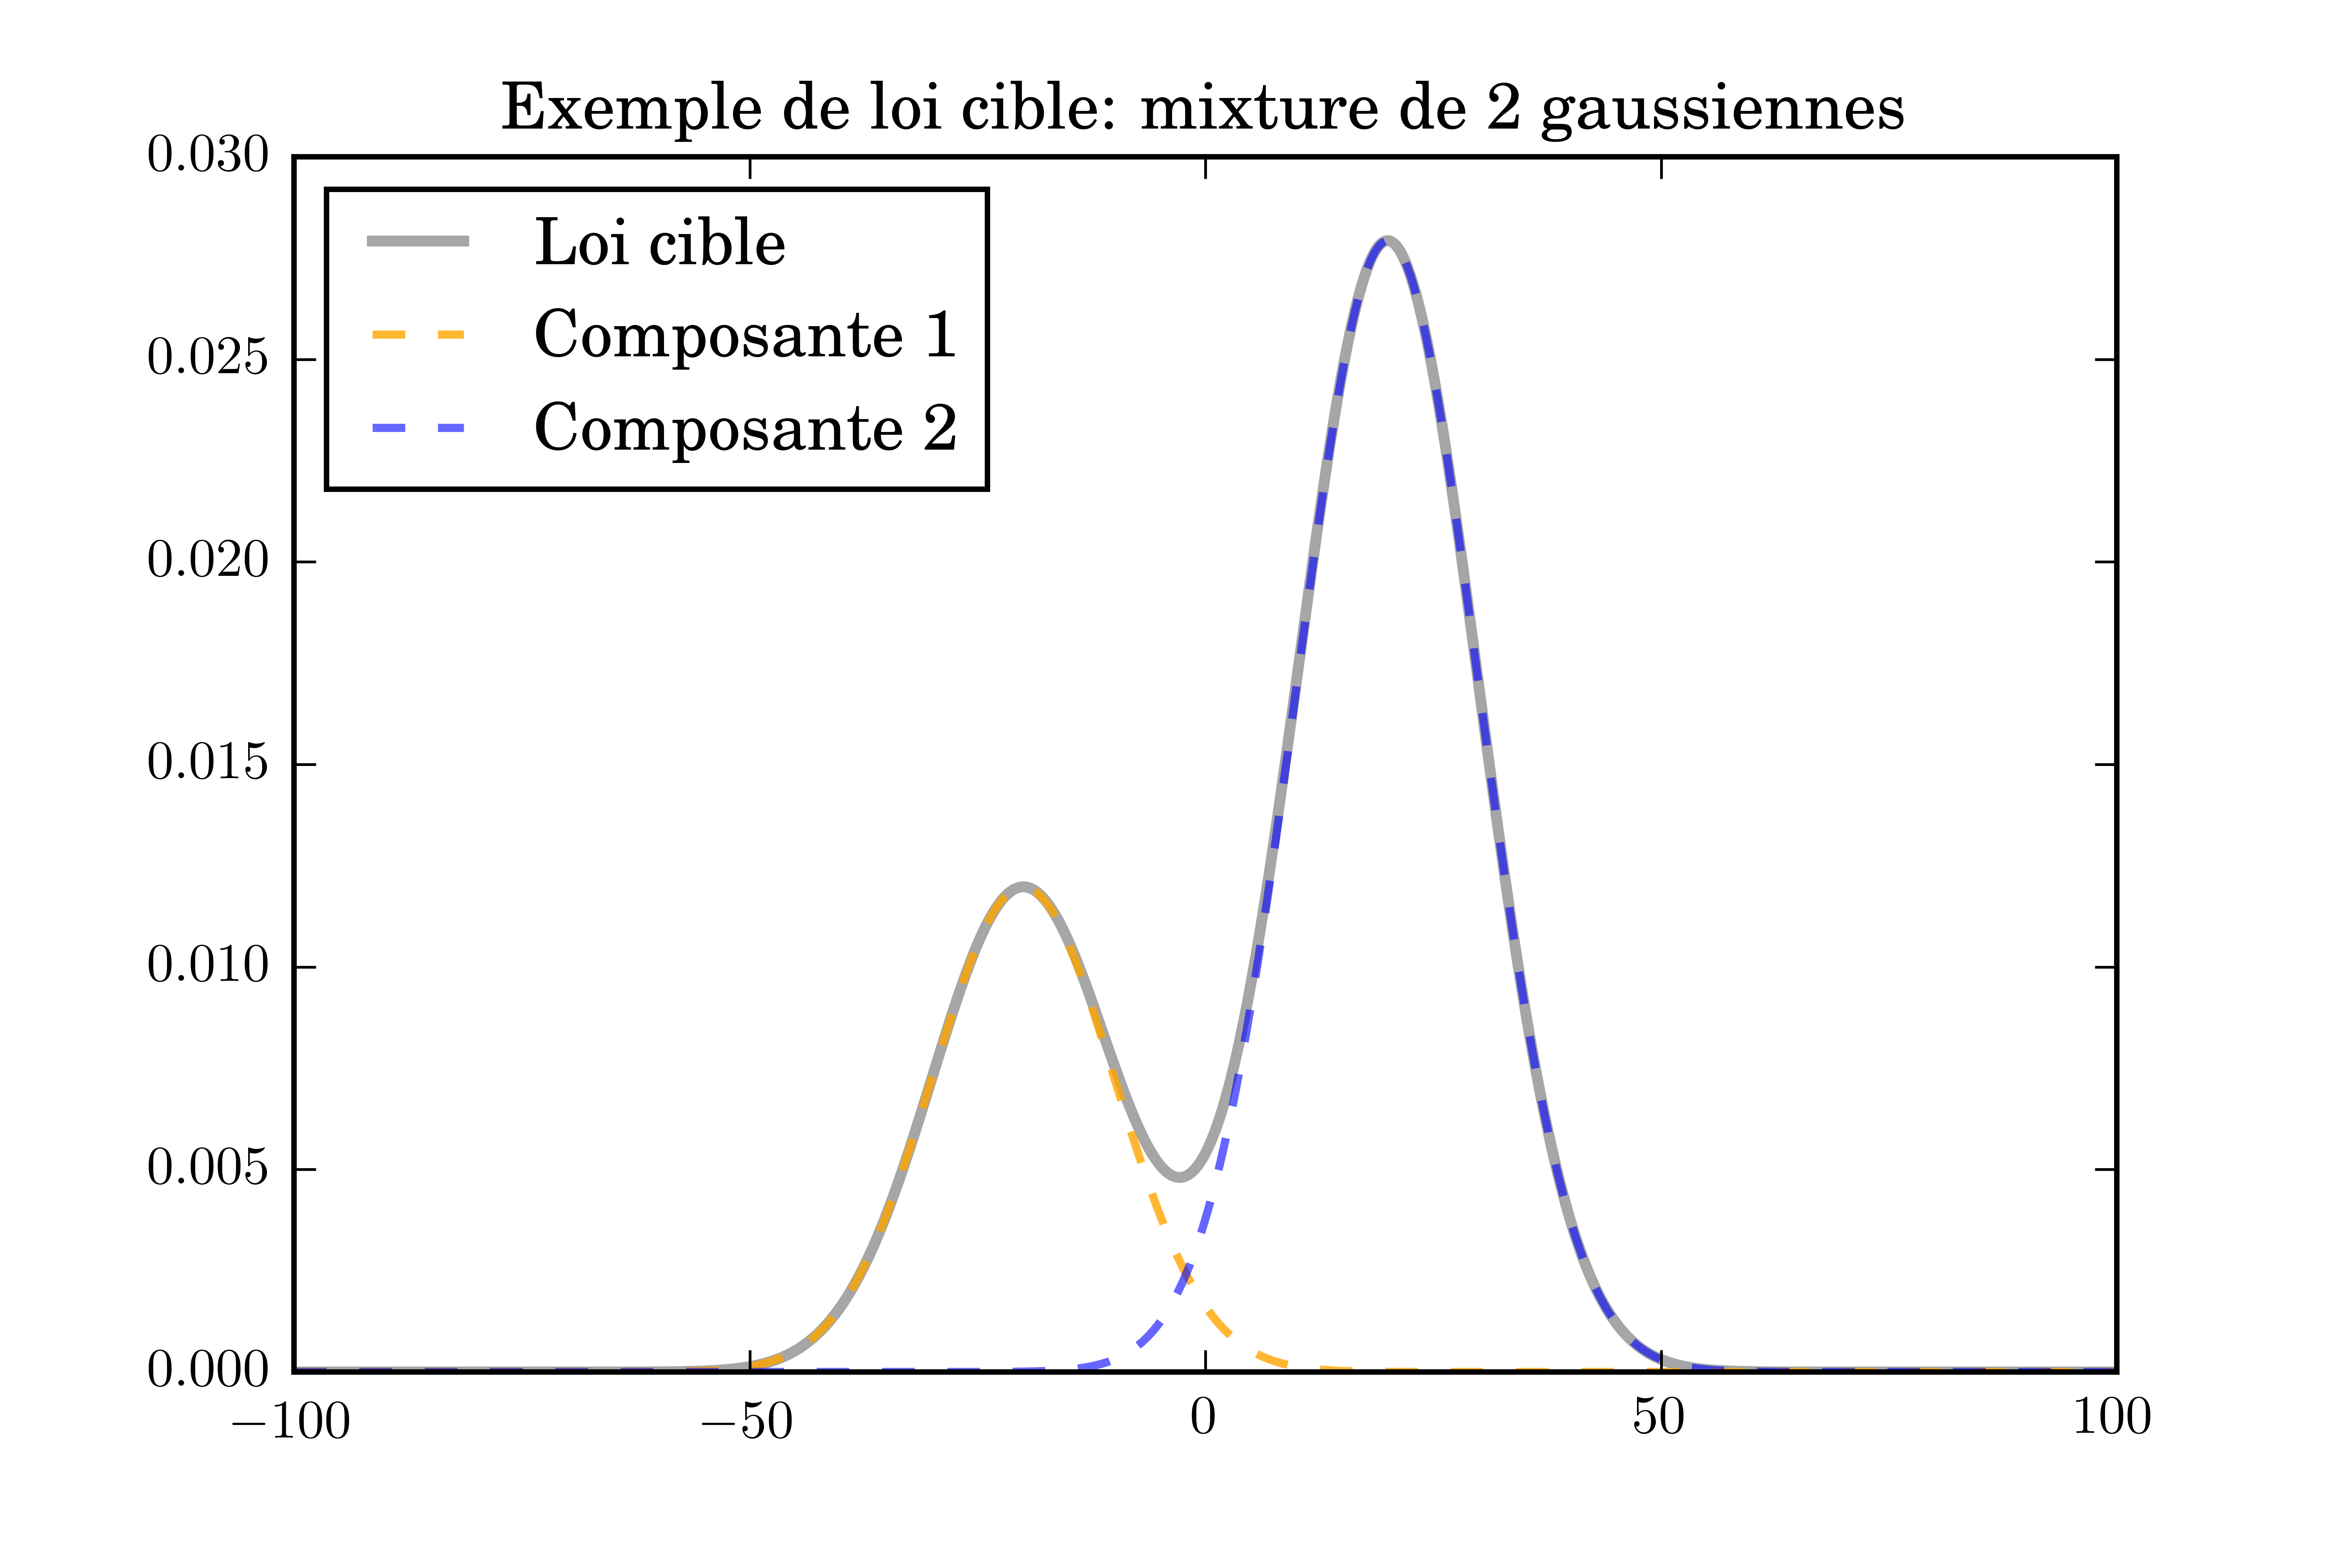
\includegraphics[scale=0.55]{courbe_pdf_mixture_1D.png}
	\caption{Exemple de loi cible: mixture de deux gaussiennes}
	\label{fig_courbe_pdf_mixture_1D}
\end{figure}


 Supposons que l'on cherche à échantillonner depuis cette distribution: nous définissons un noyau de transition de type gaussien afin d'appliquer une méthodologie de type random-walk Metropolis: 

\begin{equation}
\kernel(\VecTheta, \VecThetaCandidat ) = \mathcal{N}(\VecThetaCandidat | \VecTheta, \sigma_{K}^2)
\label{eq_noyau_gaussien}
\end{equation}

La figure \ref{fig_courbe_4_histogrammes_exemple_1} illustre ainsi l'approximation de $\pi$ grâce aux histogrammes des éléments obtenus à différentes itérations de l'algorithme. 

\begin{figure}[h!]
	\centering
	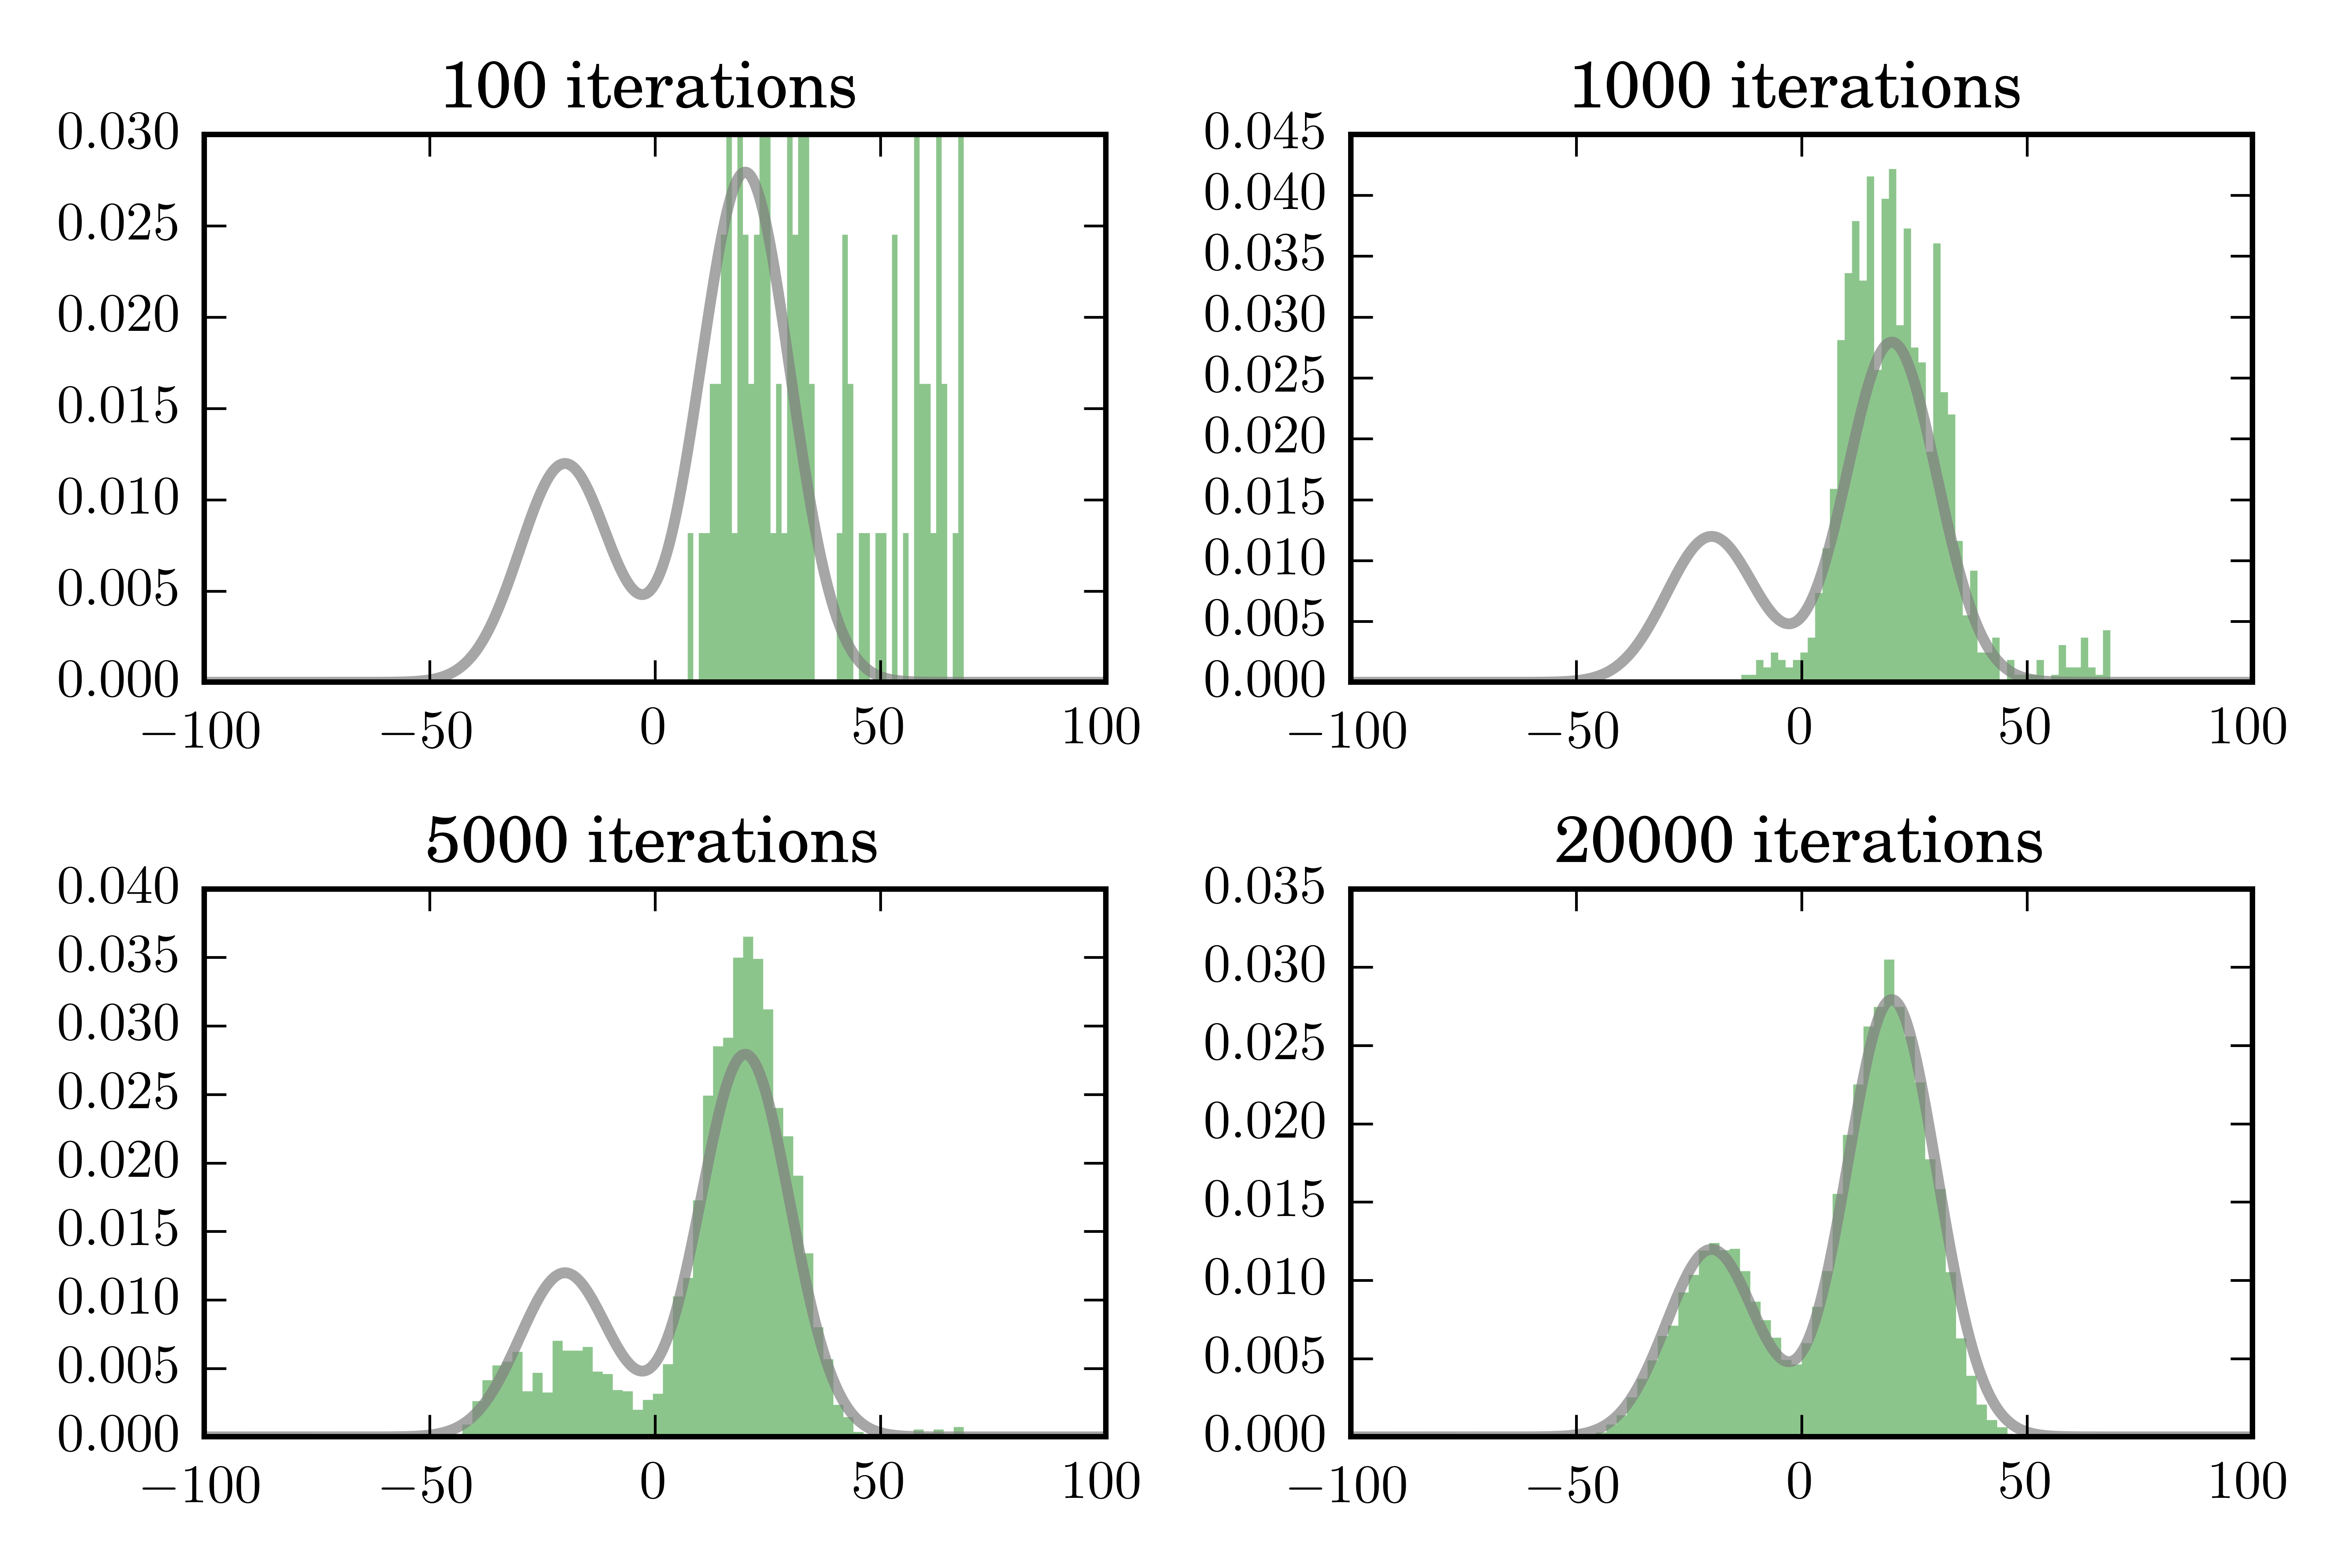
\includegraphics[scale=0.65]{courbe_4_histogrammes_exemple_1.png}
	\caption{Résultats de l'algorithme MH: histogrammes des éléments tirés (en vert) et comparaison avec la loi cible (en rouge)}
	\label{fig_courbe_4_histogrammes_exemple_1}
\end{figure}

On remarque qu'avant d'atteindre la distribution stationnaire, il existe un régime transitoire durant lequel les états de la chaîne ne permettent pas de représenter correctement la loi cible. Il est alors d'usage de ne pas tenir compte des éléments tirés durant cette période , appelée \textit{temps de chauffe} ou \textit{burn-in}. \\


\begin{figure}[h!]
	\centering
	\begin{subfigure}[t]{0.5\textwidth}
		\centering
		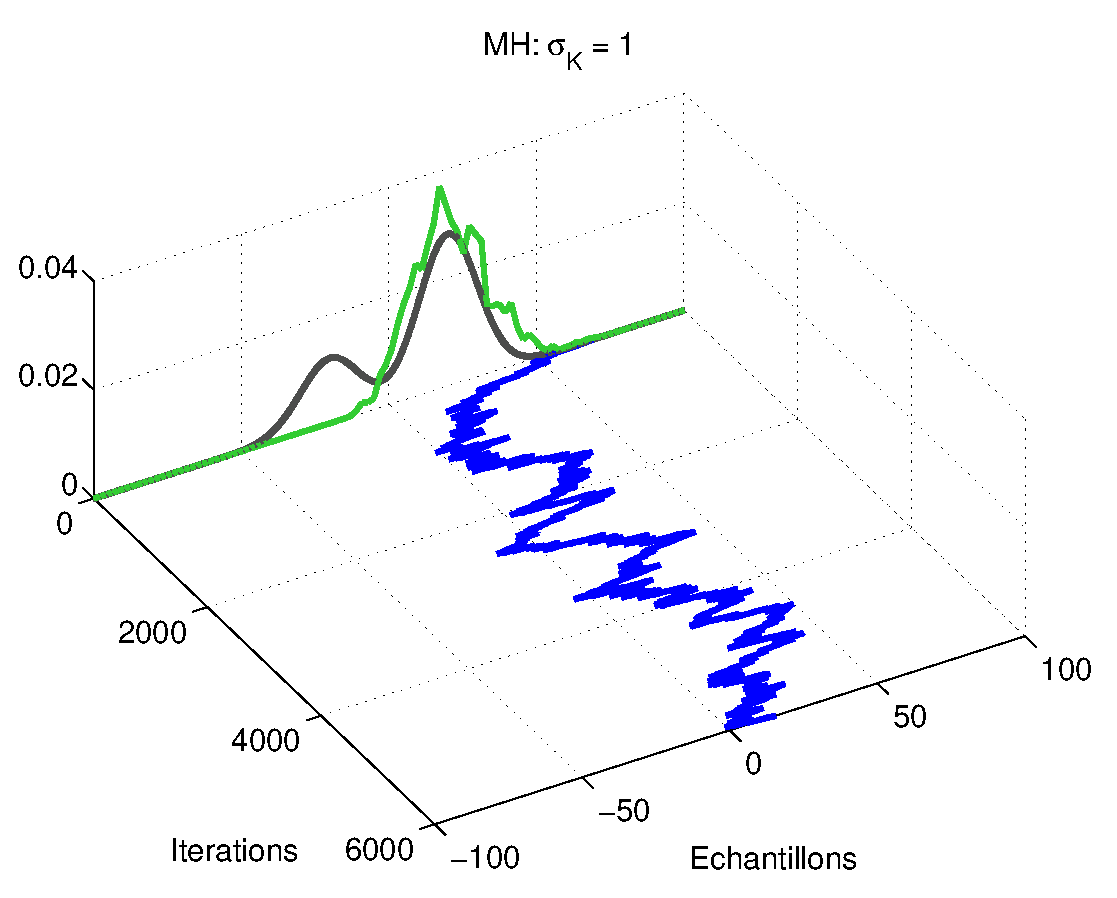
\includegraphics[width=0.9\textwidth]{courbe_MH_varKernel_1}
		\caption{}
		\label{subfig_varK_1}
	\end{subfigure}%
	~ 
	\begin{subfigure}[t]{0.5\textwidth}
		\centering
		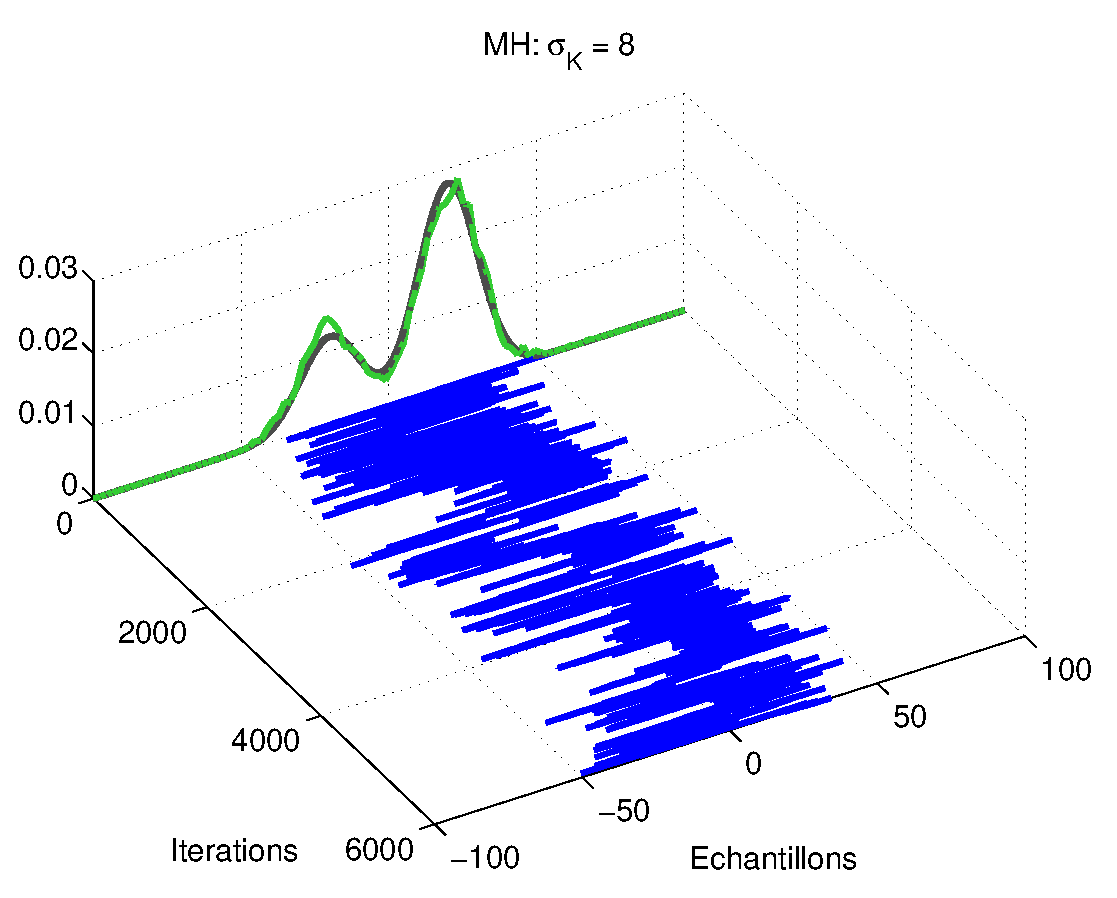
\includegraphics[width=0.9\textwidth]{courbe_MH_varKernel_8}
		\caption{}
		\label{subfig_varK_8}
	\end{subfigure}
	\begin{subfigure}{0.5\textwidth}
		\centering
		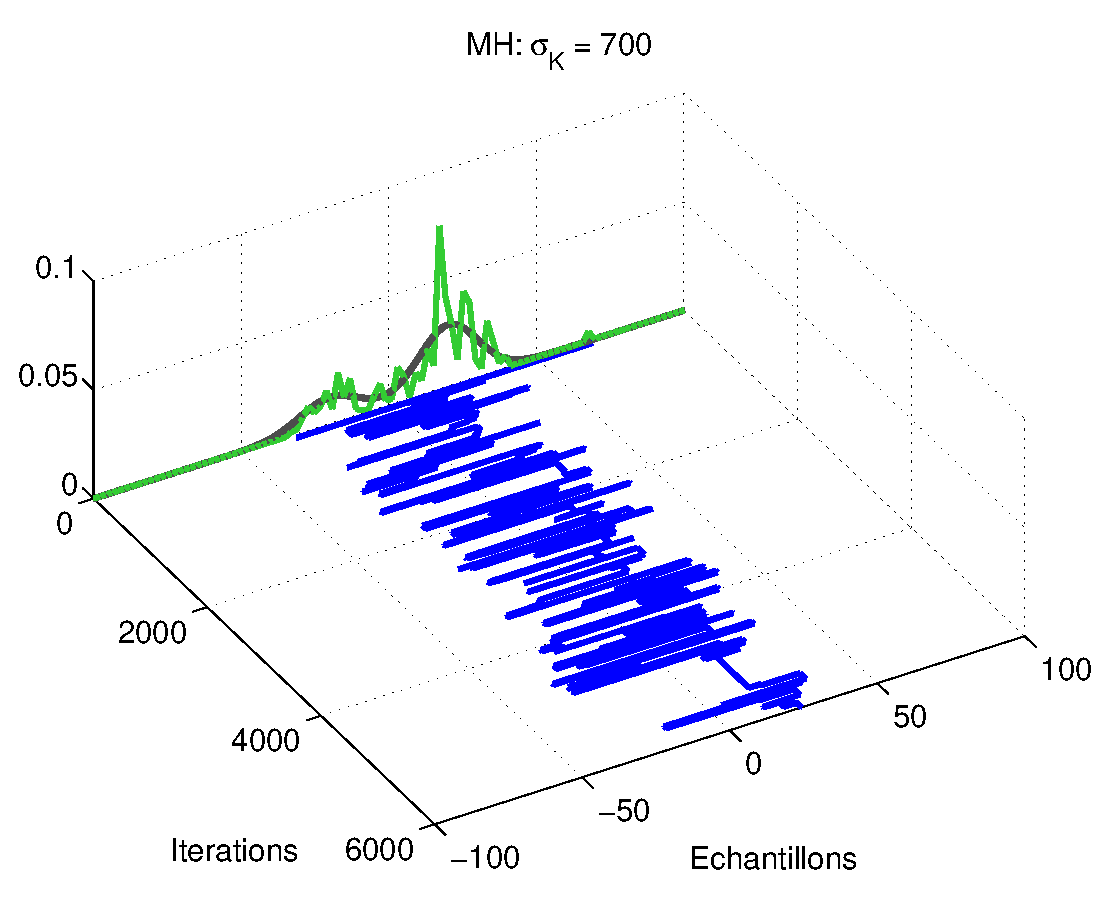
\includegraphics[width=0.9\textwidth]{courbe_MH_varKernel_700}
		\caption{}
		\label{subfig_varK_700}
	\end{subfigure}
	
	\caption{Exemples de réalisations de l'algorithme MH avec 3 valeurs différentes pour la variance du noyau de transition}
\end{figure}

La vitesse de convergence et la qualité de l'estimation sont conditionnés par deux facteurs importants: 
\begin{itemize}
	\item \textbf{l'initialisation de la chaîne}: plus l'état de départ est proche d'une valeur ayant une probabilité élevée suivant la loi cible, plus vite l'algorithme convergera. S'il est impossible de favoriser a priori une ou plusieurs valeurs de l'espace d'état, on peut simplement tirer l'état initial avec une loi uniforme sur cet espace.
	\item \textbf{le choix du noyau de transition}: dans le cas d'un random-walk Metropolis, le paramètre $\sigma_K$ reflète l'écart potentiel entre deux états consécutifs de la chaîne. Si celui-ci est trop important, les amplitudes des transitions proposées par l'algorithme deviennent trop importantes, causant un rejet fréquent des états candidats. Cela se traduit par la présence de plateaux sur la trajectoire de la chaîne, comme on le voit sur la figure \ref{subfig_varK_700}. A l'inverse, si $\sigma_K$ est choisi trop petit, l'exploration de l'espace d'état ne se fait pas de façon optimale, car la chaîne évolue beaucoup plus lentement, avec le risque de ne pas atteindre certains états représentatifs de la loi cible du fait de leur "éloignement". On retrouve ce phénomène sur la figure \ref{subfig_varK_1}, où la chaîne reste bloquée sur l'un des modes, lui empêchant d'échantillonner depuis la composante de moyenne $\mu_1 = -20$. Il faut donc choisir une valeur offrant un bon compromis, et qui permet de bien retrouver la loi cible, comme c'est le cas sur la figure \ref{subfig_varK_8}. 
\end{itemize}

\subsubsection{Echantillonneur de Gibbs}
L'échantillonneur de Gibbs a initialement été proposé dans \cite{Geman1984} puis repris et développé par \cite{Gelfand1990}. Il permet de passer du problème de l'échantillonnage d'un état $\VecTheta = (\theta_1, \dots, \theta_p)$ sur un espace pouvant être potentiellement de grande dimension, à une succession de sous-problèmes plus simples, en générant successivement chacun des éléments composant $\VecTheta$ à l'aide de leurs dépendances par rapport aux autres. C'est ainsi la loi conditionnelle de chaque élément de $\VecTheta$ sous la loi cible qui fait office de loi de proposition.

Le parcours des composantes de $\VecTheta$ peut se faire de façon déterministe, par exemple en les traitant dans leur ordre naturel les unes après les autres: on parle alors de \textit{balayage systématique}, ou \textit{systematic scan}, comme illustré dans l'algorithme \ref{algo_gibbs_sampler}. Une autre possibilité consiste à choisir aléatoirement cet ordre d'exploration: il s'agit du \textit{balayage aléatoire}, ou \textit{random scan}. \\

\IncMargin{1em}
\begin{algorithm}
	\SetAlgoLined
	Initialiser $\VecTheta^{(0)} = \left(\theta_1^{(0)}, \dots, \theta_p^{(0)}\right)$\;
	\For{$i = 1, \dots, N$ }{
		\For{$k = 1, \dots, p$}{
			Tirer $\theta_k^{(i)}$ depuis $p(\theta_k^{(i)} | \theta_1^{(i)}, \dots, \theta_{k-1}^{(i)}, \theta_{k+1}^{(i-1)}, \dots, \theta_p^{(i-1)})$
			}
		}
	\caption{Echantillonneur de Gibbs (balayage systématique)}
	\label{algo_gibbs_sampler}
\end{algorithm}

Pour illustrer le fonctionnement de ce type d'algorithme, nous allons chercher à échantillonner depuis une gaussienne bivariée à deux dimensions. Dans ce cas, on va donc noter $\VecTheta = (\theta_1, \theta_2)^T$, on a ainsi $\VecTheta \sim \mathcal{N}(\VecMu, \MatSigma)$ avec: 

\begin{equation}
\label{eq_caracs_gaussienne_bivariee}
\begin{split}
\VecMu &= (\mu_1, \mu_2)^T \\
\MatSigma &= \begin{pmatrix}
\sigma_{1}^2 & \corr_{\theta_1\theta_2} \sigma_1 \sigma_2 \\
 \corr_{\theta_1\theta_2} \sigma_1 \sigma_2 & \sigma_{2}^2 
\end{pmatrix}
\end{split}
\end{equation} 
où $\sigma_1^2$ et $\sigma_2^2$ sont les variances respectives de $\theta_1$ et $\theta_2$, et $\corr_{\theta_1\theta_2}$ est la corrélation entre $\theta_1$ et $\theta_2$ définie par: $$\corr_{\theta_1\theta_2} = \dfrac{\text{Cov}(\theta_1,\theta_2)}{\sigma_1\sigma_2}$$.

Le cas gaussien bivarié est relativement facile à traiter, car on sait calculer directement les expressions des lois conditionnelles, qui sont elle-mêmes gaussiennes, et qui s'écrivent sous la forme suivante:

 \begin{equation}
 \label{eq_conditionnelles_gaussienne_bivariee}
 \begin{split}
 p(\theta_1 | \theta_2) &= \mathcal{N}\left(\theta_1 \middle\vert \mu_1 + \sigma_1 \corr_{\theta_1\theta_2} \left(\dfrac{\theta_2 - \mu_2}{\sigma_2}\right), \sigma_1^2 (1-\corr_{\theta_1\theta_2}^2)\right) \\
 p(\theta_2 | \theta_1) &= \mathcal{N}\left(\theta_2 \middle\vert \mu_2 + \sigma_2 \corr_{\theta_1\theta_2} \left(\dfrac{\theta_1 - \mu_1}{\sigma_1}\right), \sigma_2^2 (1-\corr_{\theta_1\theta_2}^2)\right)
 \end{split}
 \end{equation}
 
\begin{figure}[h!]
	\centering
	\begin{subfigure}[t]{0.5\textwidth}
		\centering
		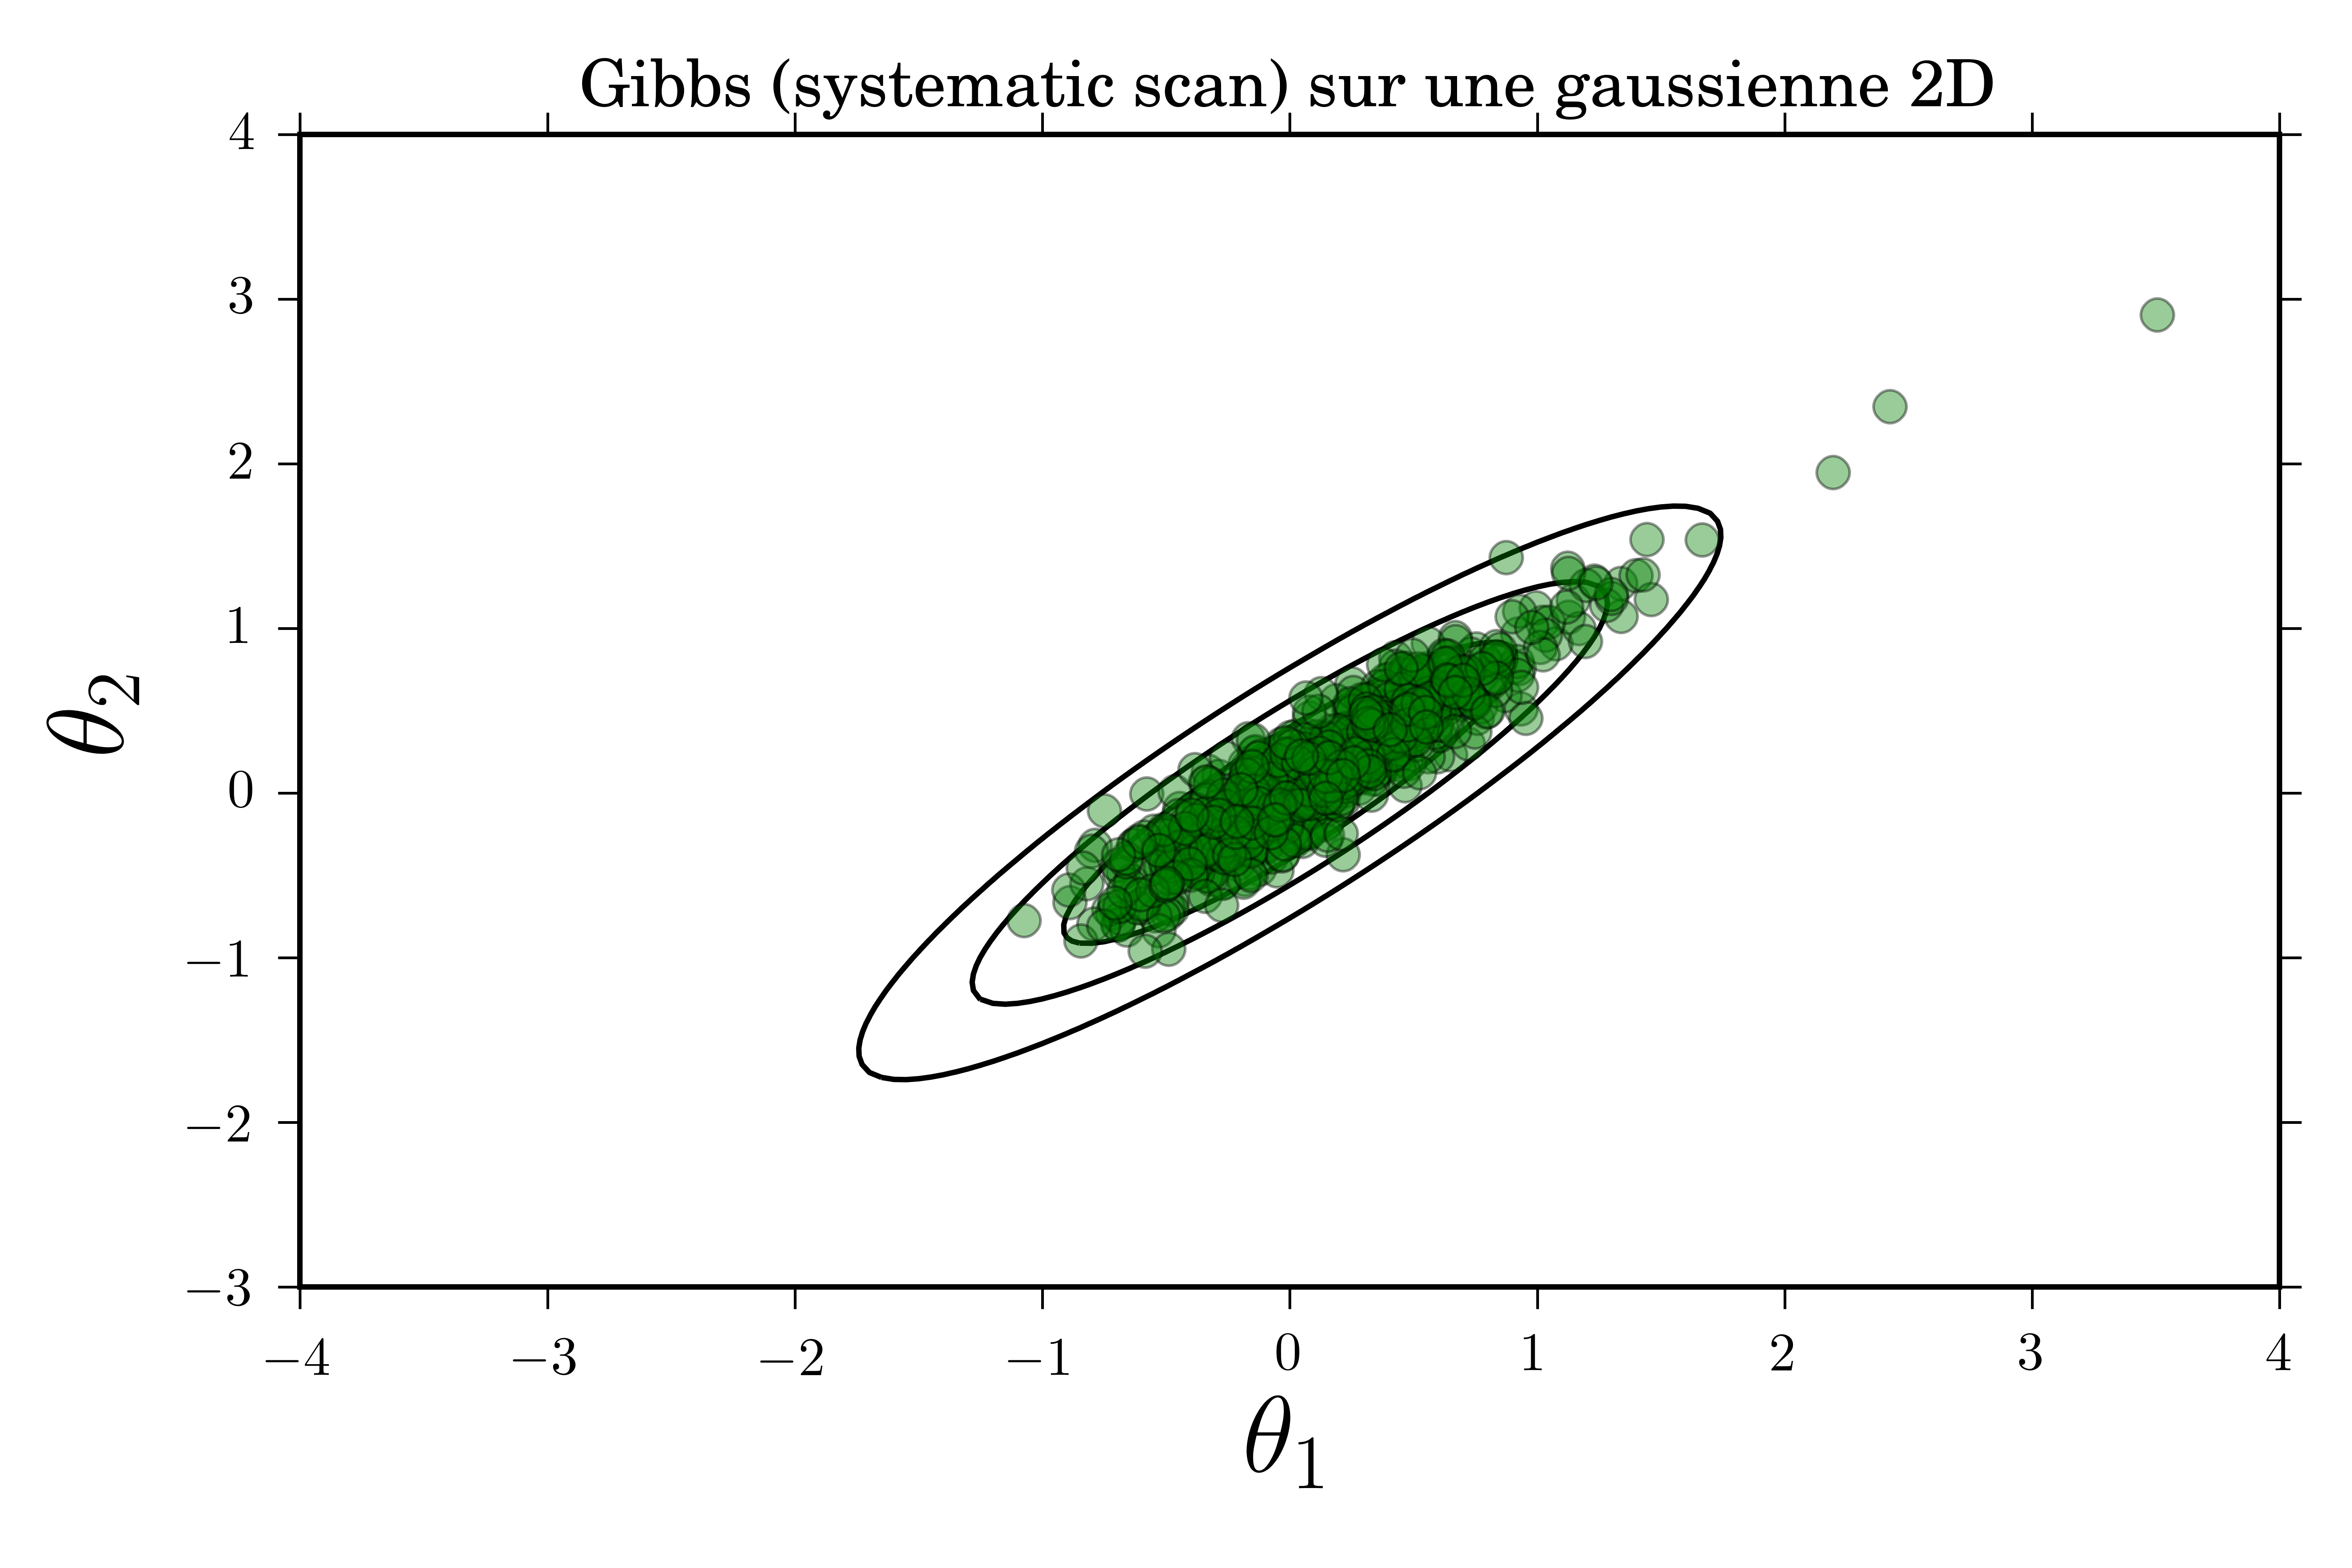
\includegraphics[width=0.9\textwidth]{courbe_gibbs_gaussienne_2D.png}
		\caption{}
		\label{subfig_gibbs_all}
	\end{subfigure}%
	~ 
	\begin{subfigure}[t]{0.5\textwidth}
		\centering
		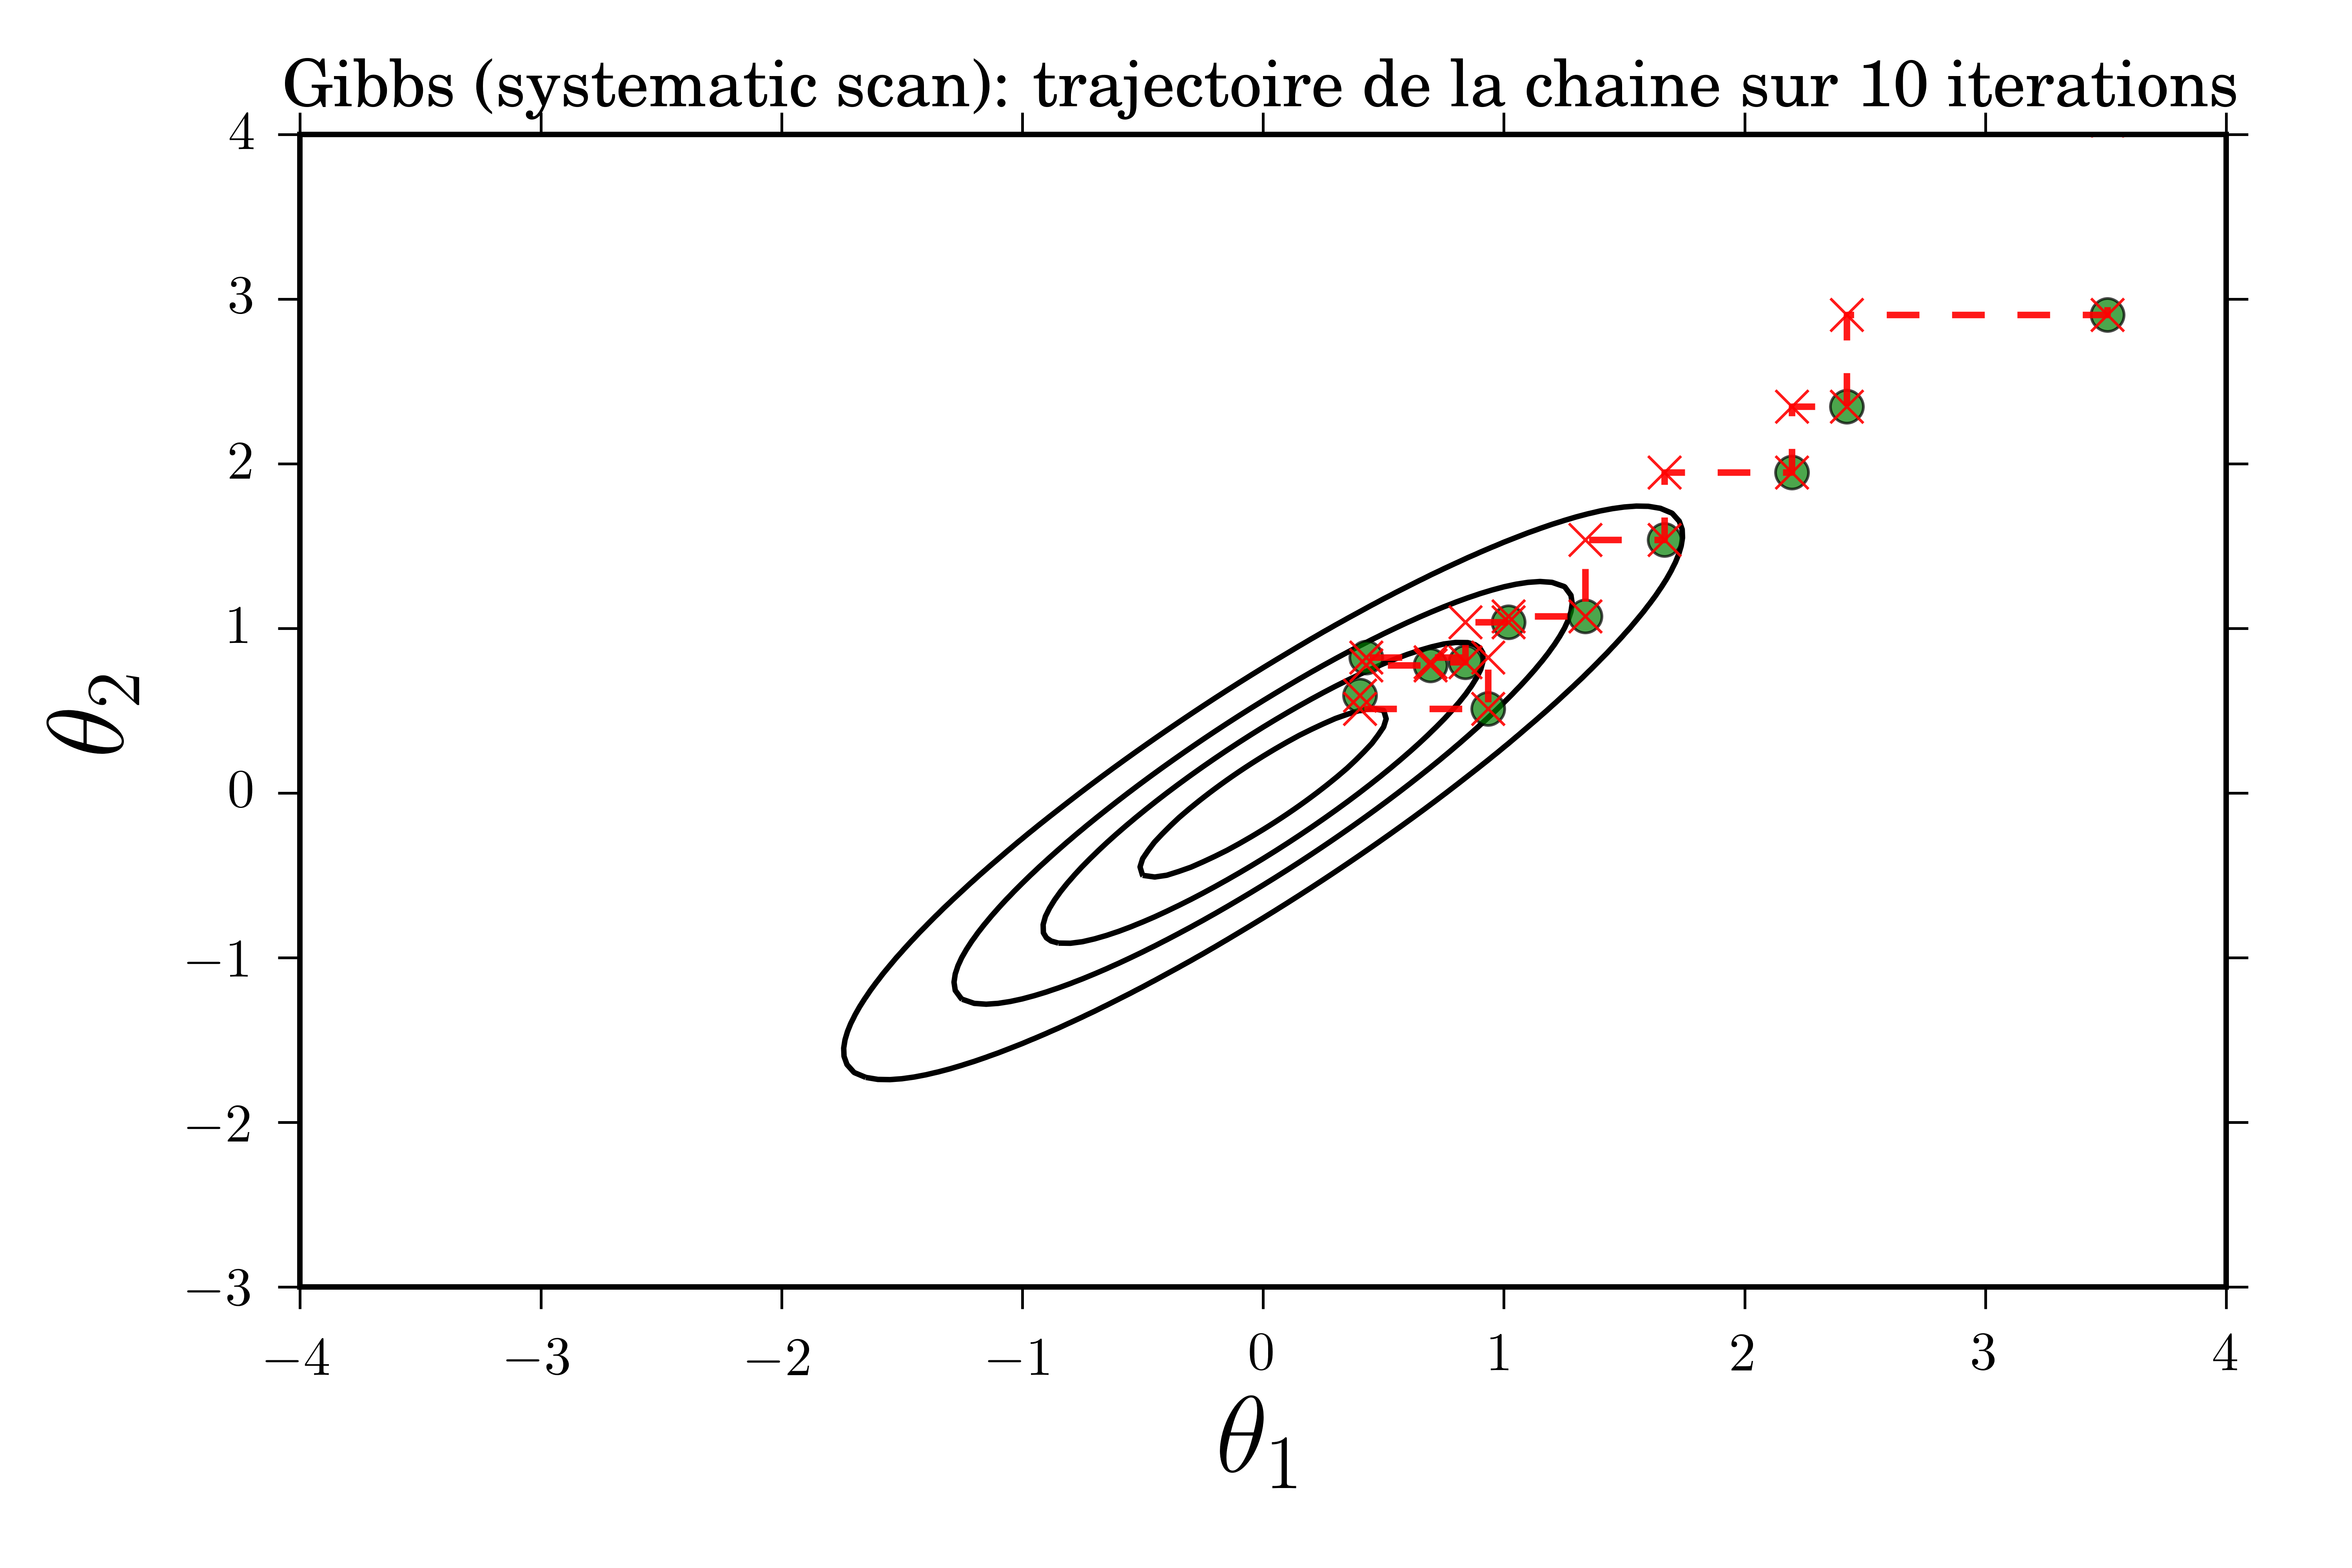
\includegraphics[width=0.9\textwidth]{courbe_gibbs_trajectoire_10_iterations.png}
		\caption{}
		\label{subfig_gibbs_10}
	\end{subfigure}
	\caption{Illustration de l'échantillonneur de Gibbs pour une loi cible de type gaussienne bivariée (en noir) avec le résultat sur 800 itérations (a) et sur 10 itérations avec trajectoire (b)}
\end{figure}

La figure \ref{subfig_gibbs_10} reflète bien le comportement de l'algorithme: la trajectoire de la chaîne (en pointillés gris) met en évidence le fait que les composantes de $\VecTheta$ sont évaluées une par une. 

Cette famille d'algorithmes, contrairement à l'approche MH, n'effectue pas de sélection des états échantillonnés, et exploite ainsi toute l'information générée lors de la simulation. Cependant, elle nécessite de pouvoir échantillonner depuis les lois conditionnelles, ce qui n'est généralement pas facile. Aussi, dans ces cas-là, une variante consiste à avoir recours à une itération de type MH avec une loi de proposition choisie par l'utilisateur: cette méthode porte le nom de \textit{Metropolis-Within-Gibbs} (MWG).\\

 
 \subsection{Echantillonnage d'importance classique (IS)}
 
 Avec les approches MCMC, on a vu qu'il existait plusieurs façons de traiter les éléments générés par la loi de proposition: on peut les soumettre à une procédure d'acceptation-rejet, ou alors tous les garder. Une autre vision du problème est proposée par les méthodes dites d'échantillonnage d'importance, ou \textit{importance sampling} (IS), où l'utilisation de poids permettent de quantifier la pertinence de chaque élément. Dans la suite de ce paragraphe, nous emploierons le terme de \textit{particules} afin de désigner les éléments d'un échantillon.\\
 
 L'idée de départ des méthodes IS est de chercher à approximer des intégrales de la forme : 
 
 \begin{equation}
  I = \mathbb{E}_\pi[f(\VecTheta)] = \int f(\VecTheta)\pi(\theta)d\VecTheta
  \label{eq_IS_integrale_1}
 \end{equation}
 
 Pour cela, on définit une loi de proposition $\propFonc$ permettant de réécrire l'équation \eqref{eq_IS_integrale_1} sous la forme:
 
 \begin{equation}
\mathbb{E}_\pi[f(\VecTheta)] = \int  f(\VecTheta) \dfrac{\pi(\theta)}{\propFonc(\VecTheta)}\propFonc(\VecTheta)d\VecTheta = \int  f(\VecTheta) w(\VecTheta) \propFonc(\VecTheta)d\VecTheta 
\label{eq_IS_integrale_2}
 \end{equation}
 où $w(\VecTheta) = \dfrac{\pi(\VecTheta)}{\propFonc(\VecTheta)}$ définit le vecteur des \textit{poids d'importance}.  La forme de l'intégrale obtenue permet alors de dire que:
 
\begin{equation}
\mathbb{E}_\pi[f(\VecTheta)] = \mathbb{E}_\propFonc[f(\VecTheta)w(\VecTheta)] 
\label{eq_IS_integrale_2_1}
\end{equation}

D'après la loi forte des grands nombres, $\sum\limits_{i=1}^N f(\VecTheta^{(i)}) w^{(i)}$ converge presque sûrement vers  $\mathbb{E}_\varphi[f(\VecTheta)w(\VecTheta)]$ pour $N \rightarrow + \infty$. En associant cela avec l'équation \eqref{eq_IS_integrale_2_1}, on obtient ainsi:
 
 \begin{equation}
 \mathbb{E}_\pi[f(\VecTheta)] \simeq I_N = \dfrac{1}{N}\sum\limits_{i=1}^N f(\VecTheta^{(i)})  w^{(i)}
 \label{eq_IS_integrale_3}
 \end{equation}
 
 Dans notre contexte, l'équation \eqref{eq_bayes_proportionnalite} nous rappelle que la loi cible n'est connue qu'à une constante près: pour en tenir compte, il est nécessaire de normaliser les poids d'importance. En écrivant : 
 
 \begin{equation}
 \forall i \in \{1, \dots, N\}, ~ \poidsNorm^{(i)} = \dfrac{w^{(i)}}{\sum\limits_{i=1}^N w^{(i)}}
 \label{eq_IS_poids_normalises}
 \end{equation}
 on garantit bien que toutes les valeurs de $\VecPoidsNorm$ sont comprises entre 0 et 1. \\
 
 En reprenant l'équation \eqref{eq_IS_integrale_3}, on peut alors obtenir une approximation de la loi cible, qui s'écrit:
 
 \begin{equation}
 \pi(\VecTheta) \simeq \sum\limits_{i=1}^N \poidsNorm(\VecTheta^{(i)})\delta_{\VecTheta^{(i)}}(\VecTheta)
 \label{eq_IS_approximation_loi_cible}
 \end{equation}

L'équation \eqref{eq_IS_approximation_loi_cible} permet ainsi d'obtenir des particules pondérées de la loi cible. Pour cela, il faut choisir une loi de proposition $\propFonc$ qui soit suffisamment proche de la loi cible, dont le support englobe celui de cette dernière, et à partir de laquelle on puisse échantillonner facilement. \\

\begin{figure}[h!]
	\centering
	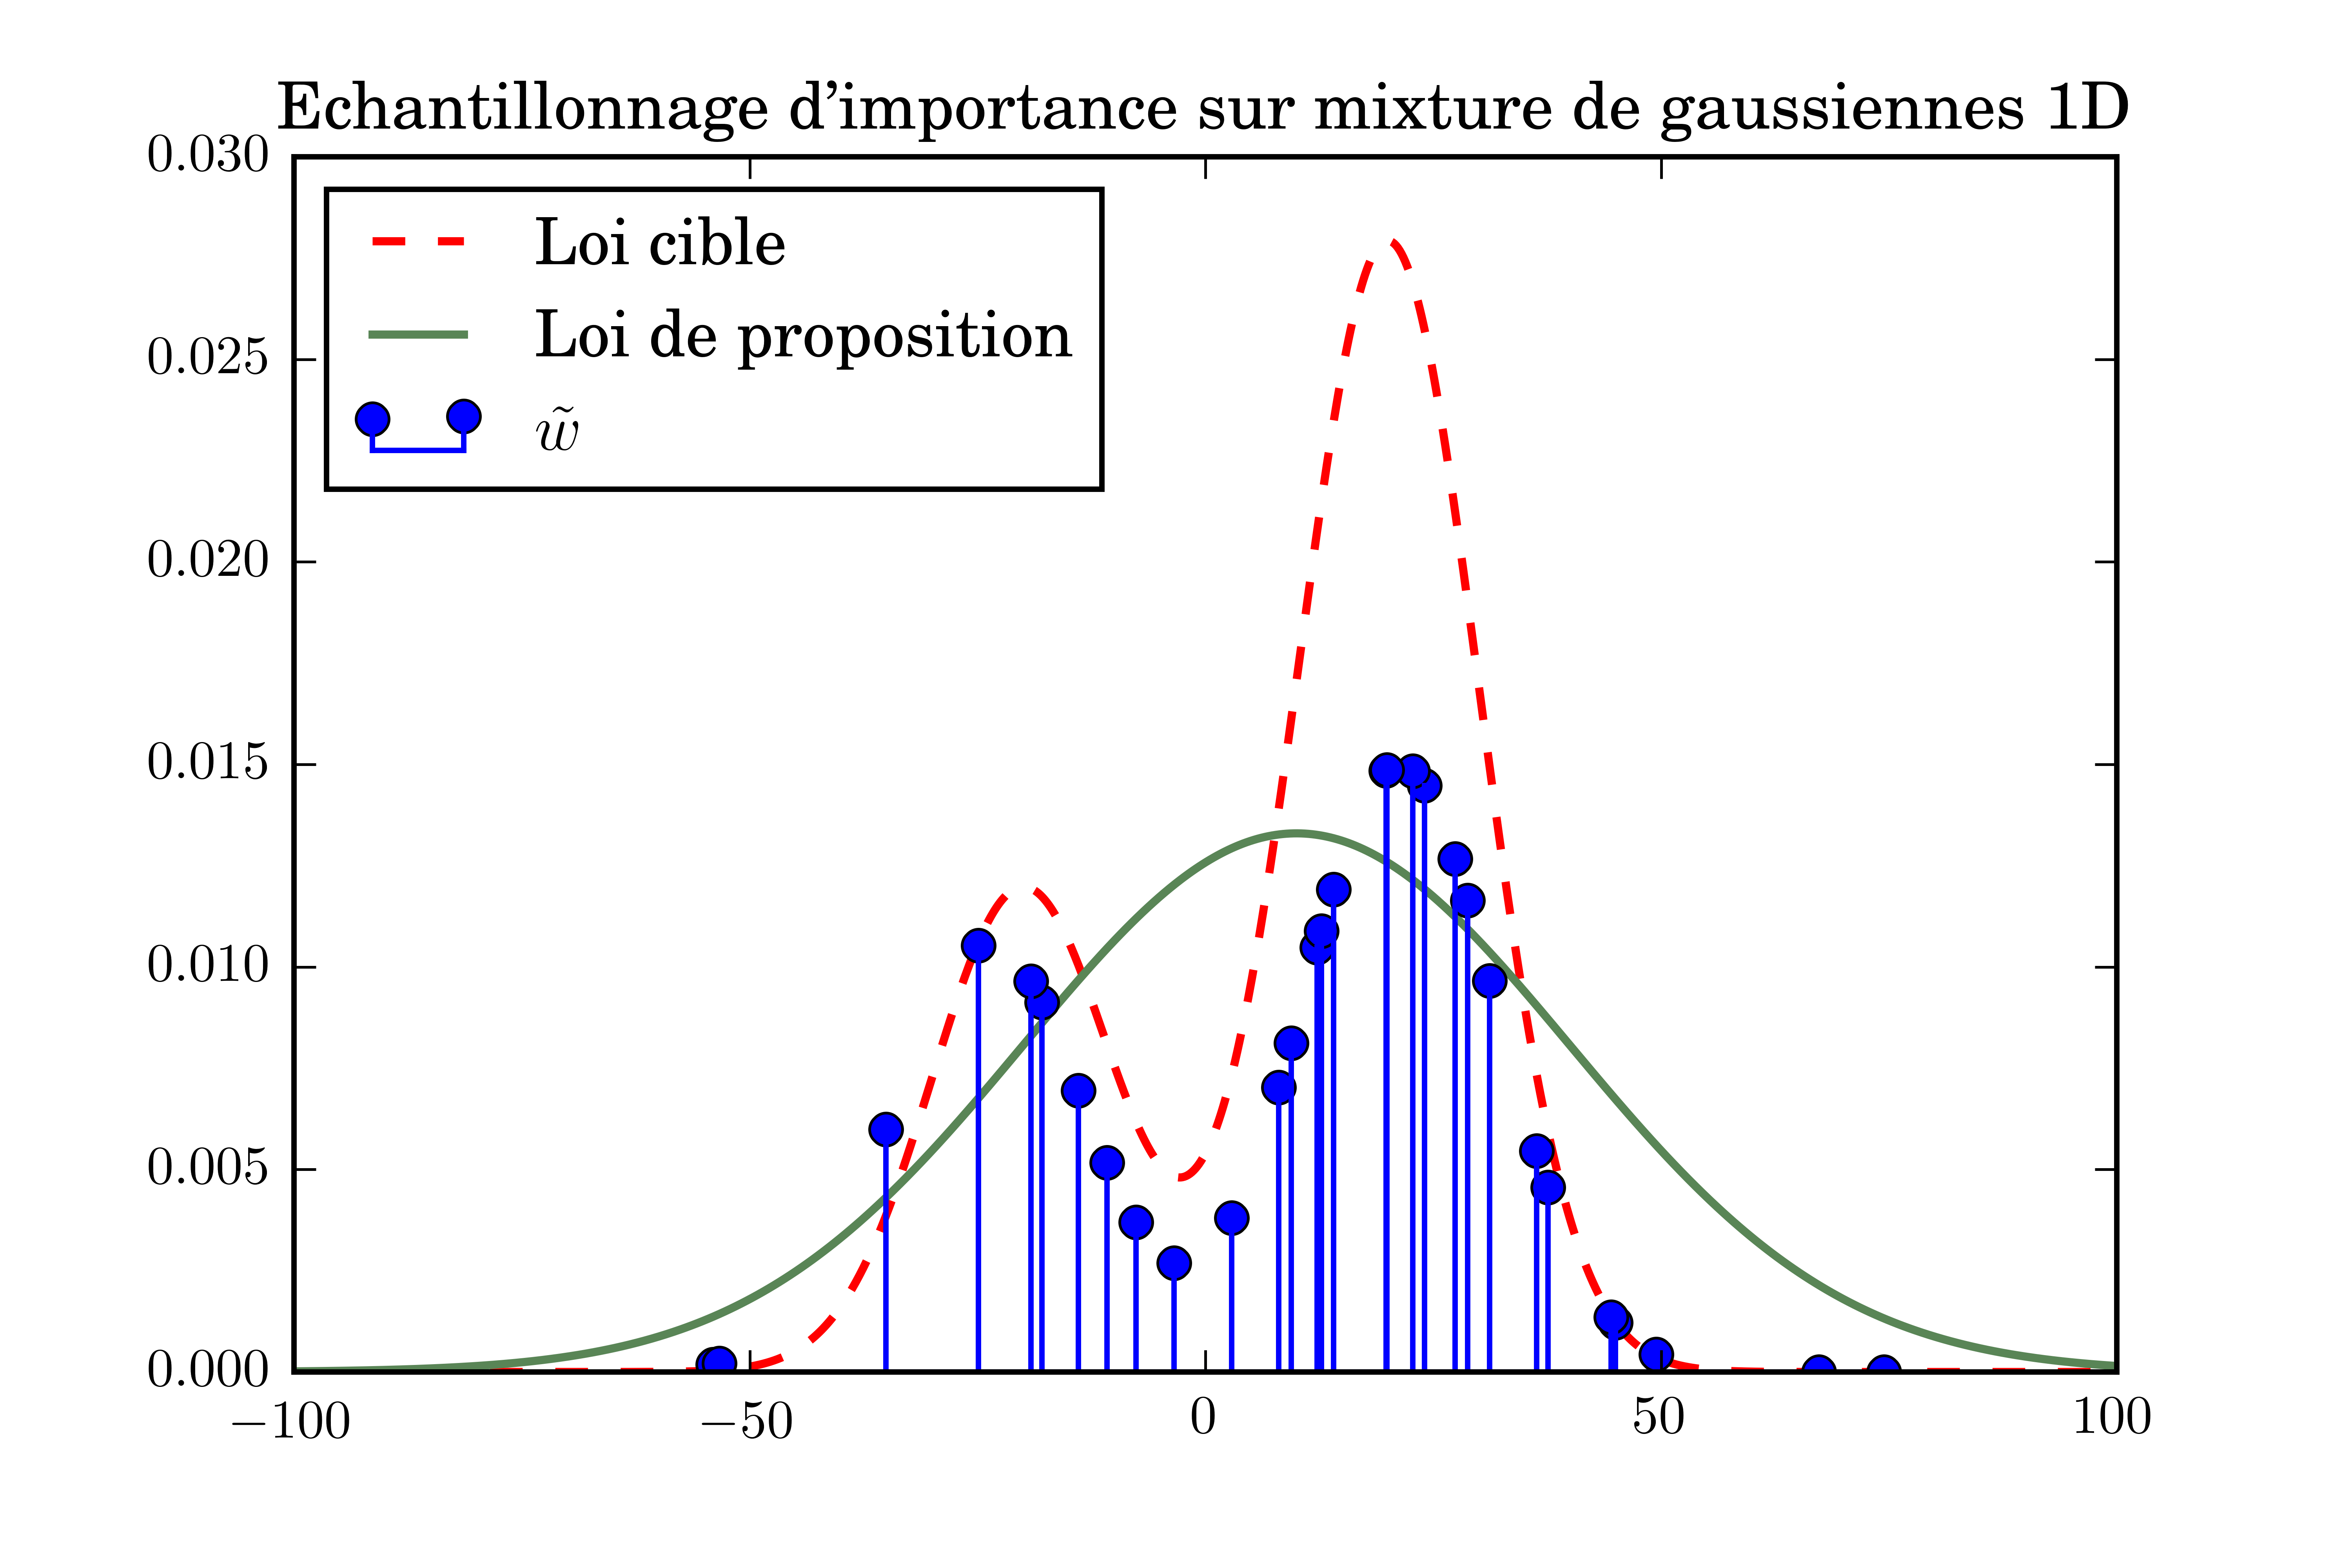
\includegraphics[scale=0.8]{courbe_IS_gmm_1D.png}
	\caption{Calcul des poids d'importance normalisés  (en bleu) sur les 30 premiers éléments d'un vecteur de 1000 particules , avec la loi cible de la figure \ref{fig_courbe_pdf_mixture_1D} (pointillés rouges) et une loi de proposition $\mathcal{N}(\mu = 10, \sigma = 30)$ (en vert).  }
	\label{fig_IS_gmm_1D}
\end{figure}

En reprenant l'exemple de la mixture de deux gaussiennes utilisé précédemment (voir équation  \eqref{eq_mixture_2_gaussiennes_1D"}), on observe sur la figure \ref{fig_IS_gmm_1D} que si la loi de proposition est bien choisie, alors on obtient une bonne approximation de la loi cible. Le choix de cette loi est en fait un point crucial des méthodes IS, et présente certaines difficultés s'il est impossible d'associer "intuitivement" une distribution $\varphi$ à une loi cible $\pi$, par exemple lorsqu'on se place dans des grandes dimensions, ou plus généralement lorsque $\pi$ est trop complexe pour être rattachée à une famille de lois connue. 

Une loi de proposition mal choisie peut engendrer un ralentissement de la convergence de l'algorithme, voire une impossibilité à approximer correctement la loi cible. Par exemple, sur la figure \ref{courbe_IS_bad_proposal}, la nouvelle loi de proposition ne permet pas d'échantillonner correctement depuis le premier mode à -20.

\begin{figure}[h!]
	\centering
	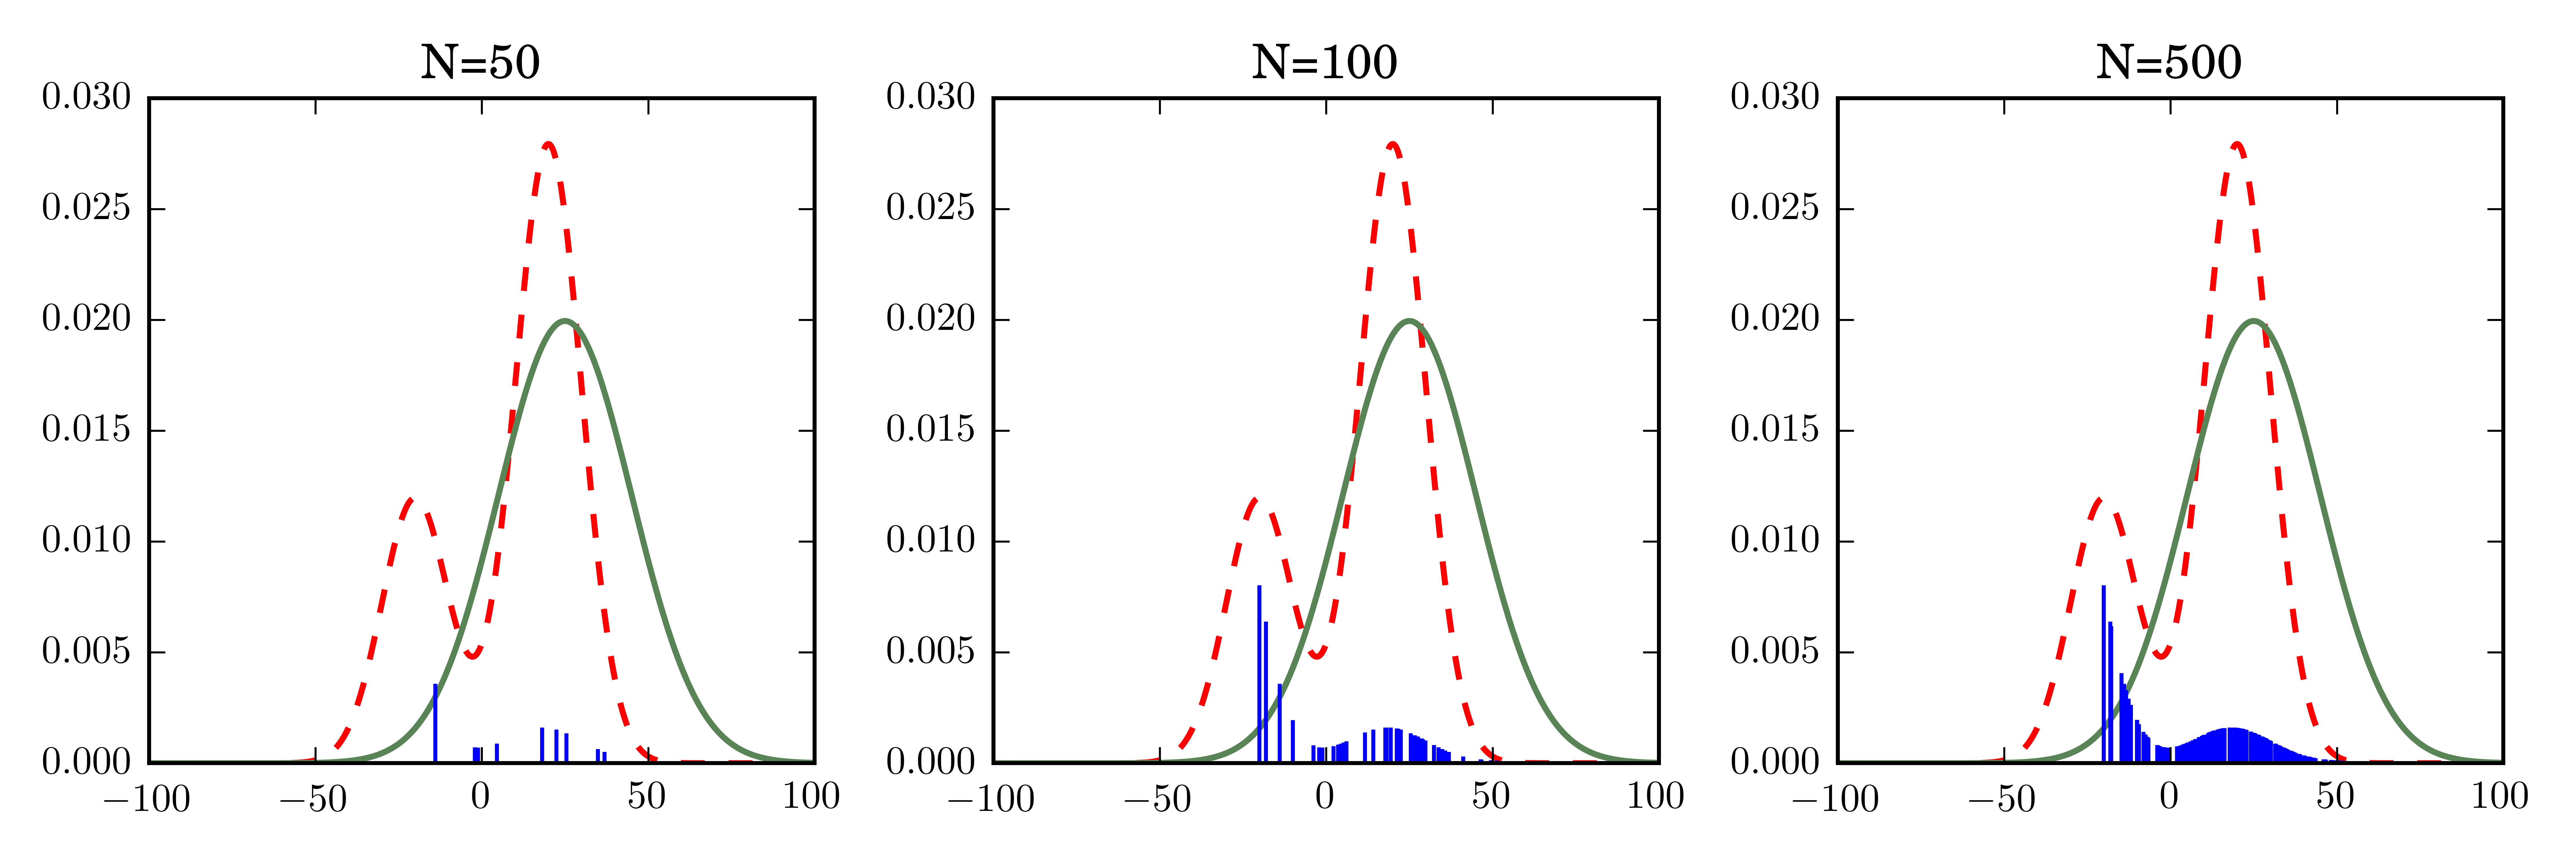
\includegraphics[width=0.99\textwidth]{courbe_IS_bad_proposal.png}
	\caption{IS pour une loi de proposition $\mathcal{N}(\mu=25, \sigma=20)$ à différentes étapes de l'échantillonnage.}
	\label{courbe_IS_bad_proposal}
\end{figure}

On observe également que les valeurs des poids des particules tirés autour du mode à -20 sont trop élevées par rapport à ce qui est attendu. On remarque aussi qu'un petit nombre de particules agrège les valeurs les plus importantes des poids, alors que la majorité restante détient des poids de faible valeur. Ce déséquilibre de répartition est plus généralement connu sous le nom de \textit{dégénérescence des poids}. La métrique permettant de quantifier ce phénomène et de facto d'évaluer les performances de la loi de proposition, est appelée \textit{Effective Sample Size} ($\ESS$), et se calcule selon la formule suivante:

\begin{equation}
\mathbb{ESS} = \dfrac{\left(\sum\limits_{i=1}^N w^{(i)}\right)^2}{\sum\limits_{i=1}^N \left(w^{(i)}\right)^2}
\label{eq_def_ESS}
\end{equation}

Dans le cas le plus extrême où une unique particule à un poids égal à 1 et toutes les autres ont un poids nul, on a $\ESS = 1$. Plus sa valeur croît, plus la loi de proposition est proche de la loi cible, le cas parfait étant $\ESS = N$ où $\propFonc$ et $\pi$ sont identiques.\\

Une façon de contourner le problème de la dégénérescence consiste à ré-échantillonner sur les points où les poids d'importance sont élevés: cette méthode fût développée par \cite{Rubin1988} sous le nom d'algorithme \textit{Sampling Importance Resampling} (SIR). Une autre alternative revient à moduler la loi de proposition en fonction des valeurs de poids obtenues, ce qui est possible grâce aux méthodes d'\textit{échantillonnage d'importance adaptatives} sur lesquelles nous allons à présent nous pencher.\\

\subsection{Méthodes d'échantillonnage d'importance adaptatif}

Le facteur-clé de la performance d'un algorithme de type IS réside dans l'utilisation d'une bonne loi de proposition: il paraît donc naturel d'envisager des méthodes permettant l'ajustement de cette loi pour qu'elle permette une bonne approximation de la loi cible. \\

\subsubsection{Population Monte Carlo}

Les travaux présentés dans \cite{Cappe2004} illustrent une première approche, appelée \textit{Population Monte Carlo} (PMC), qui peut être vue comme une version itérative de l'IS visant à adapter la loi de proposition afin de la rapprocher au mieux de la loi cible. Plus précisément, à chaque itération $k$: 
\begin{enumerate}
	\item on tire un échantillon $\VecTheta_k = (\theta_{1,k}, \dots, \theta_{N_p,k})$ de particules obtenues par une perturbation stochastique qui revient à appliquer un noyau de transition de type "marche aléatoire" sur chacun des $\theta_{1,k-1}, \dots, \theta_{N_p,k-1}$, à la façon d'une chaîne de Markov,
	\item on calcule le vecteur des poids d'importance normalisés $\VecPoidsNorm_t$ de ces particules,
	\item on génère un nouvel échantillon $(\tilde{\theta}_{1,k}, \dots, \tilde{\theta}_{N_p,k})$ obtenu par \textit{resampling} de $ (\theta_{1,k}, \dots, \theta_{N_p,k})$ en utilisant les poids $\VecPoidsNorm_k$.

\end{enumerate}

Le point 3. donne le résultat de l'algorithme à l'itération $k$, à savoir un vecteur de particules ajustées pour être proche de la loi cible. A partir de là, on peut ré-itérer en appliquant de nouveau une perturbation sur ce vecteur, et ainsi de suite. 


\subsubsection{D-kernel PMC}

\cite{Douc2007} formalise le concept d'adaptation de la loi de proposition en la définissant comme étant un mélange de $D$ noyaux fixes $\propFonc_1, \dots, \propFonc_D$ défini par : 

\begin{equation}
\propFonc_\alpha(\VecTheta, \VecThetaCandidat) = \sum\limits_{d=1}^D\alpha_d \propFonc_d(\VecTheta, \VecThetaCandidat)
\label{eq_PMC_D_Kernel}
\end{equation}
où les $\alpha_d$ définissent les \textit{facteurs d'influence} des composantes respectives $\propFonc_d$, et sont tels que $$\sum\limits_{d=1}^D \alpha_d = 1$$  La démarche proposée, portant le nom de \textit{D-kernel PMC}, consiste à ajuster les valeurs des $\alpha_d$ à chaque itération d'un algorithme PMC, sur la base d'un critère de performance visant à minimiser l'écart statistique entre la distribution de proposition et la loi cible. Un tel écart peut être quantifié par la \textit{divergence de Kullback-Leibler} (KL)  $D(\pi || \propFonc_\alpha )$, définie par : 


\begin{equation}
D(\pi || q_\alpha ) = \int \log\left(\dfrac{\pi(\VecTheta)}{q_\alpha(\VecTheta)}\right)\pi(\VecTheta)d\VecTheta
\label{eq_definition_KL}
\end{equation}

\subsubsection{M-PMC}

\cite{Cappe2008} propose une extension de ces travaux en introduisant une méthode appelée \textit{Mixture-PMC} (M-PMC) reposant sur le même type de critère de performance, mais visant cette fois à étendre la phase d'adaptation à tous les paramètres de la mixture $q_{\alpha}$, sans se limiter aux seuls $\alpha_d$ . La loi de proposition peut alors s'écrire sous la forme suivante:

\begin{equation}
\propFonc_{(\alpha,\nu)}(\VecTheta) = \sum\limits_{d=1}^D\alpha_d \propFonc_d(\VecTheta |\nu_d)
\label{eq_M_PMC_kernel}
\end{equation}
où $\nu_d$ représente les paramètres de la $d$-ième composante de la loi de proposition.

La procédure d'adaptation qui en découle s'inspire de l'algorithme dit d'\textit{Expectation-Maximization} (EM) pour construire les équations de mise à jour des éléments constituant $\nu_d$ : en effet, le fait de minimiser l'équation \eqref{eq_definition_KL} équivaut ici  à maximiser la grandeur : 

\begin{equation}
\int \log\left(\sum\limits_{d=1}^D \alpha_d \propFonc_d(\VecTheta| \nu_d)\right)\pi(\VecTheta)d\VecTheta
\label{eq_KL_pour_EM}
\end{equation} 

On se ramène ainsi à un problème similaire à celui du calcul d'un estimateur du maximum de vraisemblance pour un modèle de mixture, d'où l'emploi d'une méthode de type EM. 

Ce type de méthode est particulièrement approprié si on choisit la loi de proposition comme étant une mixture de gaussiennes multivariées, i.e. dont la densité en dimension $p$ prend la forme suivante : 

\begin{equation}
\forall d = 1, \dots, D, ~ q_d(\VecTheta|\nu_d) = \dfrac{1}{\left((2\pi)^p\det \Sigma_d\right)^{1/2}}\exp\left(-\dfrac{1}{2}(\VecTheta - \mu_d)^T \Sigma_d^{-1}(\VecTheta - \mu_d)\right)
\label{eq_def_multivariate_gaussian}
\end{equation}
où $\nu_d = (\mu_d, \Sigma_d)$ représente les paramètres classiques (moyenne et matrice de covariance) de la $d$-ième composante. En effet, dans ce cas-là, les équations de mise à jour de $\nu_d$ peuvent être obtenues de façon analytique. Pour cela, en se plaçant à l'itération $k$ sur la $d$-ième composante et pour la $i$-ème particule, on définit tout d'abord la grandeur intermédiaire suivante:

\begin{equation}
	\rho_d^k(\VecTheta_k^{(i)} | \alpha_d^k , \nu_d^k) = \dfrac{\alpha_d^k \varphi_d(\VecTheta_k^{(i)} | \nu_d^k)}{\sum\limits_{m=1}^D\alpha_m^k \varphi_d(\VecTheta_k^{(i)} | \nu_m^k)}, ~~ i \in \{1, \dots, N\}
\end{equation}

La mise à jour de $\alpha_d^k$ et des éléments $\mu_d^k$ et $\Sigma_d^k$ de $\nu_d^k$ est alors donnée par:

\begin{equation}
\begin{split}
\alpha_d^{k+1}  &= \sum\limits_{i=1}^N \tilde{w}_k^{(i)} \rho_d^k(\VecTheta_k^{(i)} | \alpha_d^k , \nu_d^k) \\
\mu_d^{k+1} &= \dfrac{\sum\limits_{i=1}^N\tilde{w}_k^{(i)} \rho_d^k(\VecTheta_k^{(i)} | \alpha_d^k , \nu_d^k) \VecTheta_k^{(i)}}{\alpha_d^{k+1} } \\
\Sigma_d^{k+1} &= \dfrac{\sum\limits_{i=1}^N \tilde{w}_k^{(i)} \rho_d^k(\VecTheta_k^{(i)} | \alpha_d^k , \nu_d^k)(\VecTheta_k^{(i)} - \mu_d^{k+1})(\VecTheta_k^{(i)} - \mu_d^{k+1})^T }{\alpha_d^{k+1}}
\end{split}
\label{eq_maj_gaussien}
\end{equation}


Une démonstration de ces résultats est détaillée dans \cite{Bilmes1998}. \\


A chaque itération $k \in {1, \dots, K}$, l'approche M-PMC permet ainsi, à partir des particules échantillonnées depuis la loi de proposition courante et de leurs poids d'importance respectifs, d'obtenir la nouvelle proposition $\propFonc_{\alpha^{k+1}, \nu^{k+1}}$ qui sera réutilisée à l'itération suivante. Contrairement à la version originale du PMC, ici le tirage des nouvelles particules ne dépend plus directement des anciennes, qui ne sont pas explicitement considérées comme des paramètres de la loi de tirage. \\

\subsubsection{Adaptive Multiple Importance Sampling (AMIS)}

Dans le cas du M-PMC, un problème qui peut se poser est celui de la persistance d'un ou plusieurs poids à forte valeur. En effet, si lors d'une itération on observe un phénomène de dégénérescence, celui-ci va subsister tout au long du schéma itératif, et risque de fausser les calculs du fait de la nature adaptative de la démarche, qui réutilise tous les poids existants, et ni la mise à jour des paramètres de la loi de proposition, ni la normalisation du vecteur des poids d'importance ne règle le problème. Cela se traduit alors concrètement par une variance systématiquement élevée de la distribution des poids d'importance, et peut alors conduire  à de mauvais résultats d'estimation. \\

Une façon d'y remédier est proposée dans \cite{Veach1995} et \cite{Owen2000} avec l'utilisation d'une méthode appelée \textit{deterministic multiple mixture}. En pratique,cela consiste à modifier la formule de calcul du poids d'importance $w_k^{(i)}$ associé à la particule $\theta_k^{(i)}$ à l'itération $k$. Le but est de prendre en compte la suite $(\propFonc_0, \dots, \propFonc_k)$ des distributions de proposition, et non plus uniquement la loi  courante $\propFonc_k$. Pour cela, on définit la grandeur suivante:
\begin{equation}
\vartheta_k^{(i)} = N_p \propFonc_{\alpha^0,\nu^0}(\theta_k^{(i)}) + \sum\limits_{l=1}^k N_p \propFonc_{\alpha^l,\nu^l}(\theta_k^{(i)})
\label{eq_DMW_1}
\end{equation}

On peut alors écrire la nouvelle formule permettant de calculer le poids d'importance $w_k^{(i)}$:

\begin{equation}
w_k^{(i)} = \dfrac{\pi(\theta_k^{(i)})}{\left(\dfrac{1}{(k+1)N_p}\vartheta_k^{(i)}\right)} = (k+1)N_p\dfrac{\pi(\theta_k^{(i)})}{\vartheta_k^{(i)}}
\end{equation}

Ce cheminement peut être appliqué à la fois pour le calcul du poids courant, mais également pour ajuster les poids calculés lors des itérations précédentes: on parle alors de \textit{recyclage des poids}. Un tel processus de stabilisation  permet ainsi d'atténuer automatiquement les valeurs des poids d'importance sujets à dégénérescence en les pénalisant par rapport aux poids obtenus aux itérations suivantes.\\

Le fait de coupler au sein d'un même algorithme : \\

\begin{itemize}
	\item le  recyclage optimal des poids d'importance générés entre le début de la simulation et l'itération courante,
	\item la mise à jour des paramètres de la loi de proposition en fonction des poids d'importance,\\
\end{itemize}
constitue ainsi le coeur des travaux présentés dans \cite{Cornuet2012}, qui ont mené à la création de l'algorithme d'\textit{Adaptive Multiple Importance Sampling} (AMIS). \\

L'AMIS permet donc de ré-exploiter toutes l'information disponible (sur les poids et les lois de proposition) de façon optimale, son fonctionnement est détaillée dans l'algorithme \ref{algo_AMIS}. 

\IncMargin{1em}
\begin{algorithm}
	\SetAlgoLined
	\SetKwInOut{Input}{Entrées}
	\SetKwInOut{Output}{Sorties}
	
	\Input{Les paramètres $\alpha^0$, $\nu^0$ de la loi de proposition initiale $\propFonc_{\alpha^0, \nu^0}$}
	
	Générer $N_p$ particules $\valTheta_0^{(1)}, \dots, \valTheta_0^{(N_p)}$ depuis  $\propFonc_{\alpha^0, \nu^0}$\\
	\For{$i=1, \dots, N_p$}{
		Calculer les poids d'importance initiaux:\\
		$\vartheta_0^{(i)} = N_p \propFonc_{\alpha^0, \nu^0}(\valTheta_0^{(i)})$\\
		$w_0^{(i)} = \dfrac{\pi(\theta_0^{(i)})}{\propFonc_{\alpha^0, \nu^0}(\theta_0^{(i)})}$\\
		}
	Normaliser les poids initiaux:\\
	\For{$i=1, \dots, N_p$}{
		$\tilde{w}_0^{(i)} = \dfrac{w_0^{(i)}}{\sum\limits_{j=1}^{N_p}w_0^{(j)}}$
		}
	Mettre à jour la loi de proposition en calculant $\alpha^1$ et $\nu^1$ à partir de $\alpha^0$, $\nu^0$ et $\tilde{w}_0$ \\
	\For{$k=1, \dots, K$}{
		Générer $N_p$ particules $\theta_k^{(1)}, \dots, \theta_k^{(N_p)}$ depuis la loi de proposition courante $\propFonc_{\alpha^k, \nu^k}$:\\
		\For{$i=1, \dots, N_p$}{
			Calculer les poids d'importance de l'échantillon courant:\\
			$\vartheta_k^{(i)} = N_p \propFonc_{\alpha^0, \nu^0}(\theta_k^{(i)}) + \sum\limits_{l=1}^k N_p \propFonc_{\alpha^l, \nu^l}(\theta_k^{(i)})$\\
			$w_k^{(i)} = (k+1)N_p \dfrac{\pi(\theta_k^{(i)})}{\vartheta_k^{(i)}} = (k+1)N_p \dfrac{p(\VecObs | \theta_k^{(i)})p(\theta_k^{(i)})}{\vartheta_k^{(i)}}$
			}
		Recycler les poids des particules obtenues par les précédentes lois de proposition :\\
		\For{$l=0, \dots, k-1$}{
			\For{$i=1, \dots, N_p$}{
				$\vartheta_l^{(i)} = \vartheta_l^{(i)} + N_p \propFonc_{\alpha^k, \nu^k}(\theta_l^{(i)})$\\
				$w_l^{(i)} = (k+1) N_p \dfrac{\pi(\theta_l^{(i)})}{\vartheta_l^{(i)}}$
				}
			}
		Normaliser les poids recyclés et courants:
		\For{$l=0, \dots, k$}{
			\For{$i=1, \dots, N_p$}{
				$\tilde{w}_l^{(i)} = \dfrac{w_l^{(i)}}{\sum\limits_{l'=1}^k\sum\limits_{j=1}^{N_p} w_{l'}^{(j)}}$
				}
			}
		Mettre à jour la loi de proposition en calculant $\alpha^{k+1}$ et $\nu^{k+1}$ à partir de $\alpha^k$, $\nu^k$ et de la concaténation des poids recyclés normalisés $\tilde{w}_0, \dots, \tilde{w}_k$\\
		}
		\Output{ La collection de toutes les particules: $\theta_0^{(1)}, \dots, \theta_0^{(N_p)}, \theta_1^{(1)}, \dots, \theta_K^{(1)}, \dots, \theta_K^{(N_p)}$
			
		ainsi que les poids recyclés associés:\\
		  $\tilde{w}_0^{(1)}, \dots, \tilde{w}_0^{(N_p)}, \tilde{w}_1^{(1)}, \dots, \tilde{w}_K^{(1)}, \dots, \tilde{w}_K^{(N_p)}$}
	

	\caption{Adaptive Multiple Importance Sampling (AMIS)}
	\label{algo_AMIS}
\end{algorithm}

\subsubsection{Exemple d'application de l'AMIS}

Afin d'illustrer le fonctionnement et les résultats de l'AMIS, nous reprenons le cas du mélange de gaussiennes présenté à l'équation \eqref{eq_mixture_2_gaussiennes_1D}. Supposons qu'on dispose d'un vecteur d'observations $\Vecy$ suivant cette distribution, avec $\sigma_1 = \sigma_2 = 1$ et $\gamma = 0.3$. Le vecteur $\VecTheta = (\mu_1, \mu_2)$ des moyennes de chaque composante du mélange constitue l'inconnue à estimer.\\

Si on formule le problème sous sa forme bayésienne, celui-ci peut s'écrire sous la forme suivante:
\begin{equation}
	\pi(\VecTheta) = p(\VecTheta | \Vecy) \propto p(\Vecy | \VecTheta) p(\VecTheta)
	\label{eq_bayes_ex_amis}
\end{equation}

On choisit un a priori gaussien sur chacune des composantes, de moyenne 1 et de variance 10. Comme $\mu_1$ et $\mu_2$ sont indépendants, on a :

\begin{equation}
	p(\VecTheta) = p(\mu_1)p(\mu_2)
\end{equation}

La loi de vraisemblance est obtenue grâce au modèle de mélange de l'équation \eqref{eq_mixture_2_gaussiennes_1D}: 

\begin{equation}
	p(\Vecy | \VecTheta) = \gamma \mathcal{N}(\Vecy | \mu_1,\sigma_1^2) + (1-\gamma)\mathcal{N}(\Vecy | \mu_2, \sigma_2^2)
\end{equation}

Comme il est impossible d'obtenir une forme analytique de la loi a posteriori \eqref{eq_bayes_ex_amis}, nous passons par l'algorithme AMIS pour en obtenir une approximation. Pour cela, on choisit une loi de proposition gaussienne bi-variée, suffisamment flexible et dont il est facile d'obtenir des échantillons:

\begin{equation}
\varphi(\VecTheta) = \mathcal{N}(\VecTheta | \Vecmup, \MatSigmap)
\end{equation}

On initialise cette loi de proposition avec $\Vecmup^{(0)} = (1,1)$ et $\MatSigmap^{(0)} = \begin{pmatrix} 20&0\\ 0&20 \end{pmatrix}$ pour bien couvrir l'espace des paramètres à explorer. \\

En reprenant l'algorithme \ref{algo_AMIS} et en l'appliquant à notre exemple, on peut décomposer l'exécution de l'AMIS en plusieurs étapes caractéristiques. Ainsi, à l'itération $k$:

\begin{enumerate}
	\item on échantillonne depuis la loi de proposition courante afin d'obtenir un ensemble de $N$ particules : 
	$$ \VecTheta_k^{(1)}, \dots, \VecTheta_k^{(N)} \sim \varphi (\Vecmup^k, \MatSigmap^k) $$
	
	\item on calcule $\vartheta_k$ et le vecteur des poids d'importance pour l'itération courante $w_k$
	
	\item on recycle les poids générés aux itérations précédentes
	
	\item  on met les paramètres de la loi de proposition à jour: comme on est dans un cadre gaussien, on peut reprendre les équations \ref{eq_maj_gaussien}, on a alors : 
	\begin{equation*}
	\begin{split}
		\Vecmup^{k+1} &= \sum\limits_{i=1}^N \tilde{w}_k^{(i)}\VecTheta_k^{(i)} \\
		\MatSigmap^{k+1} &= \sum\limits_{i=1}^N \tilde{w}_k^{(i)}(\VecTheta_k^{(i)} - \Vecmup^{k+1} )
(\VecTheta_k^{(i)} - \Vecmup^{k+1} )^T	\end{split}
	\end{equation*}
\end{enumerate}

Au bout de $K$ itérations, l'approximation de la loi a posteriori est ainsi donnée par : 

\begin{equation}
\pi(\VecTheta) \simeq \sum\limits_{k=1}^K \sum\limits_{i=1}^N \tilde{w}_k^{(i)} \VecTheta_k^{(i)}
\end{equation}

\begin{figure}[h!]
	\centering
	\begin{subfigure}[t]{0.5\textwidth}
		\centering
		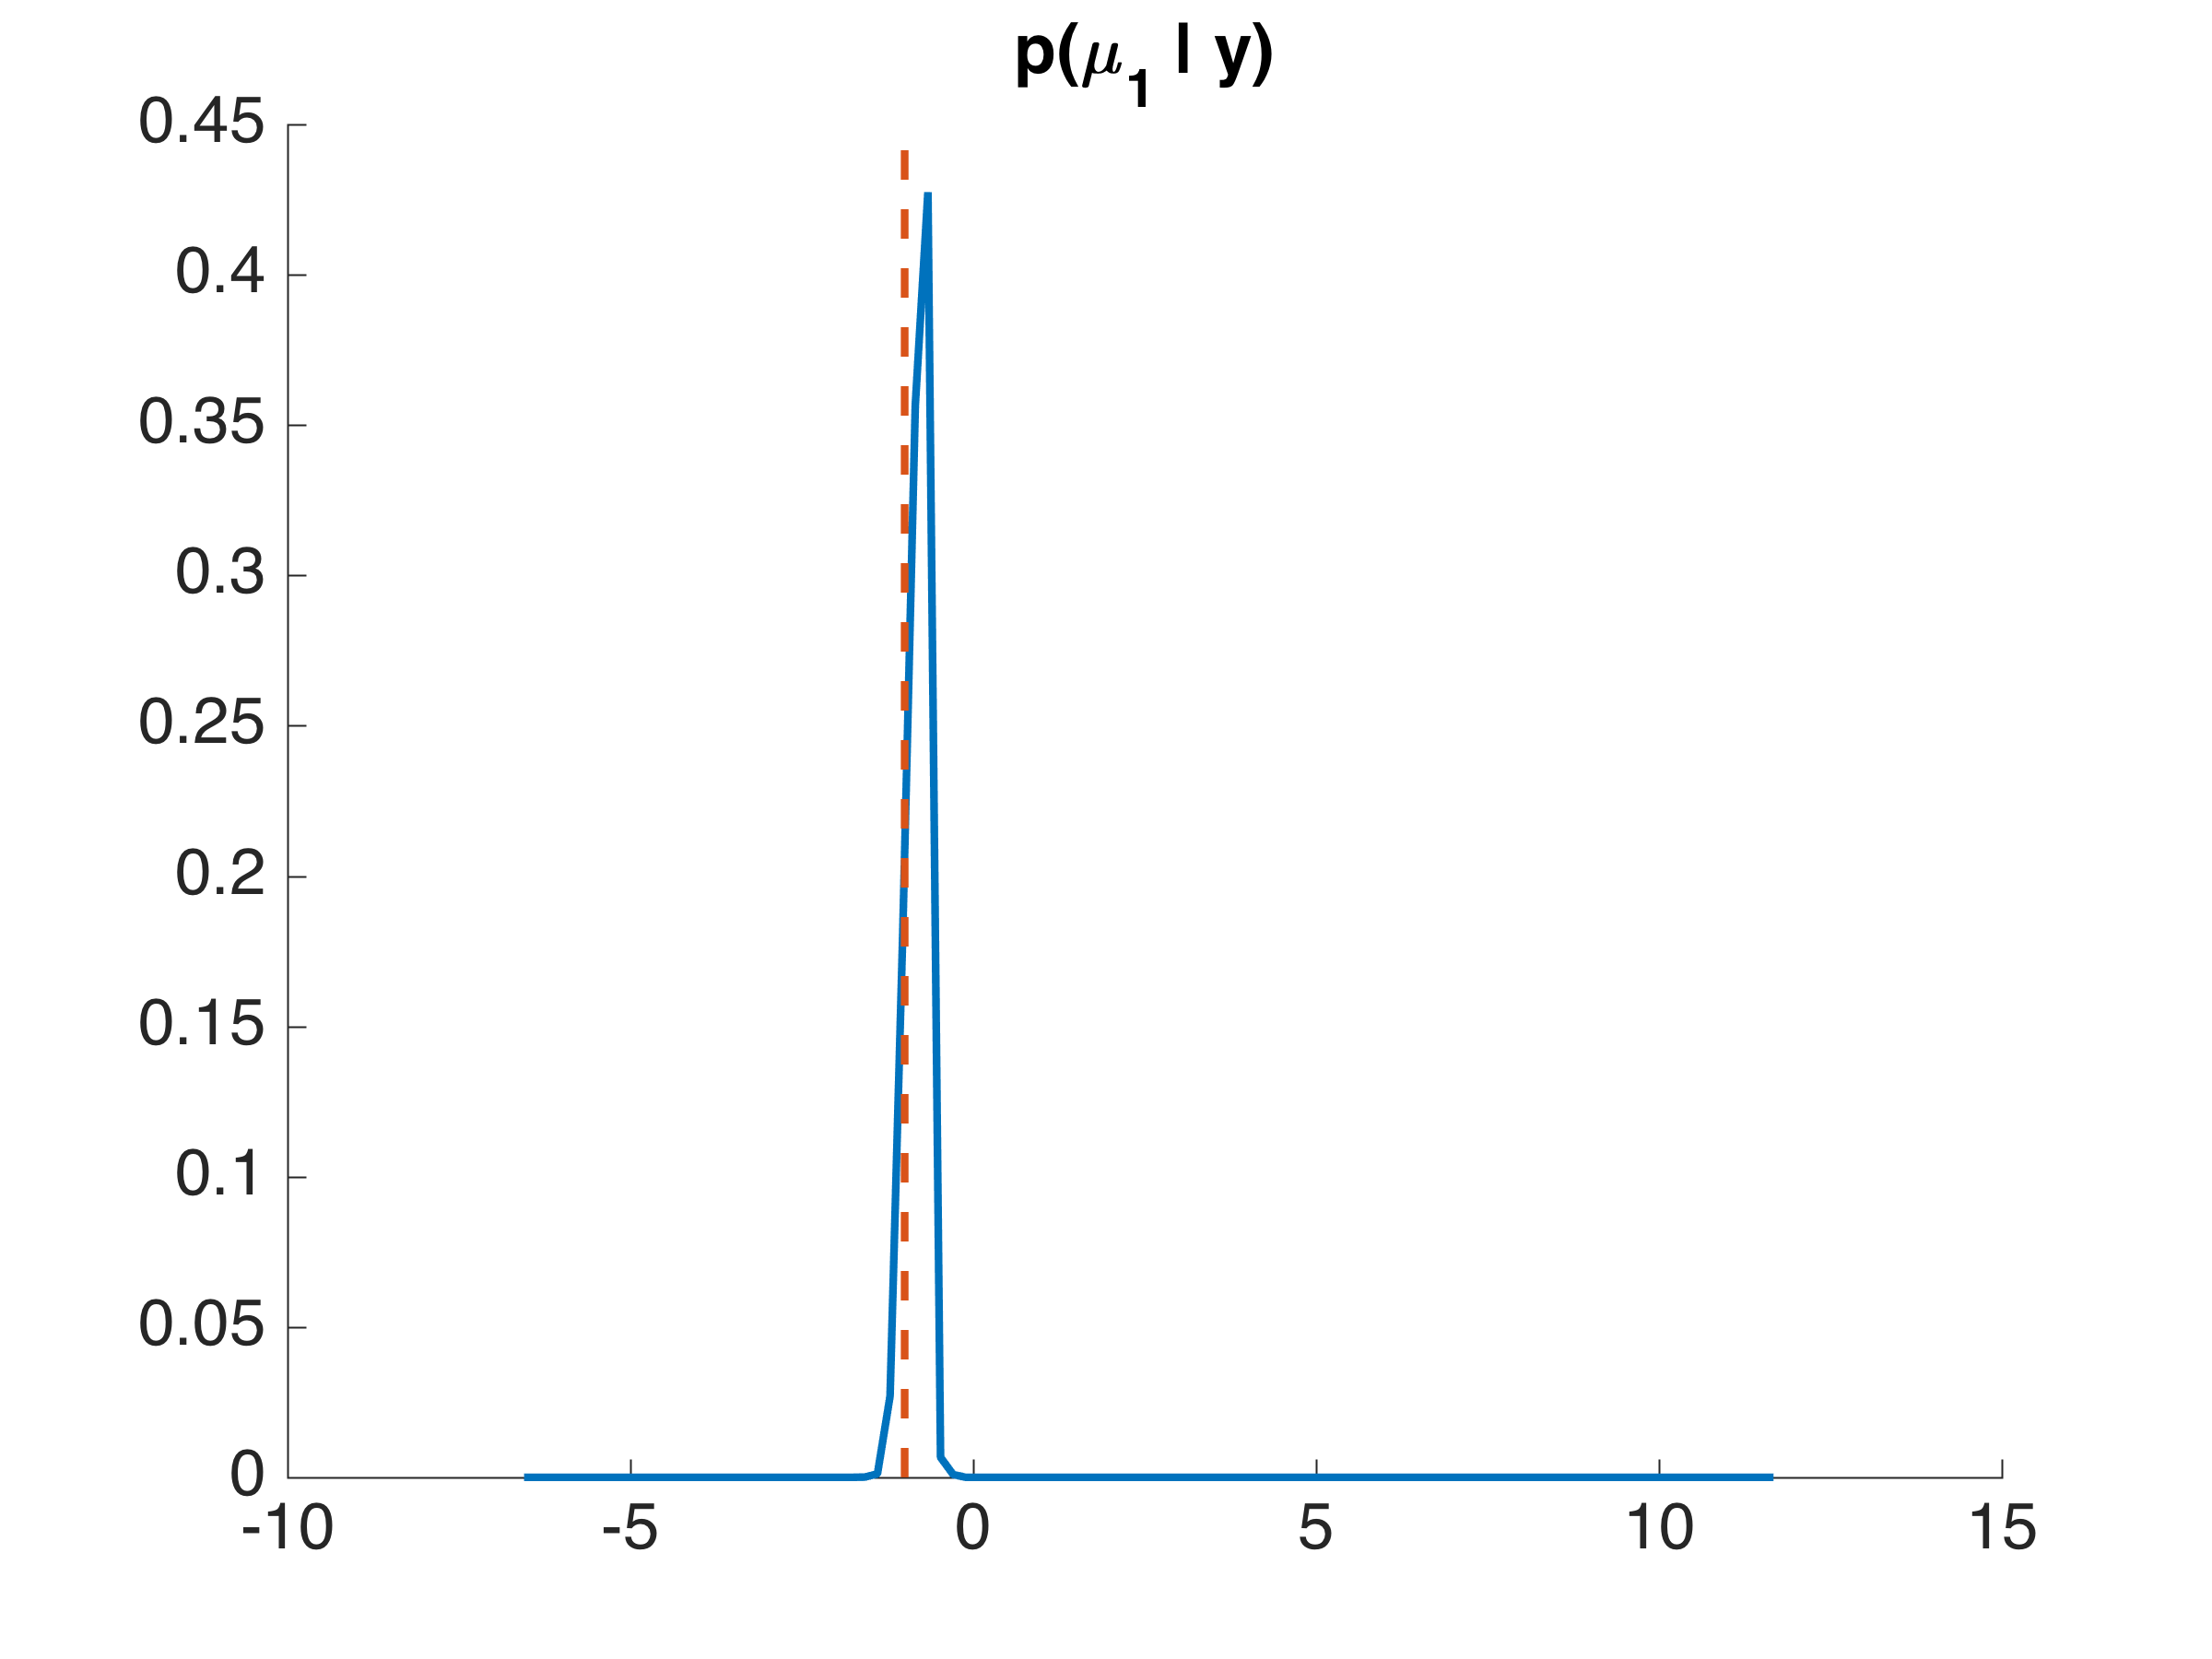
\includegraphics[width=0.9\textwidth]{posterior_mu1}
		\caption{}
		\label{posterior_mu1}
	\end{subfigure}%
	~ 
	\begin{subfigure}[t]{0.5\textwidth}
		\centering
		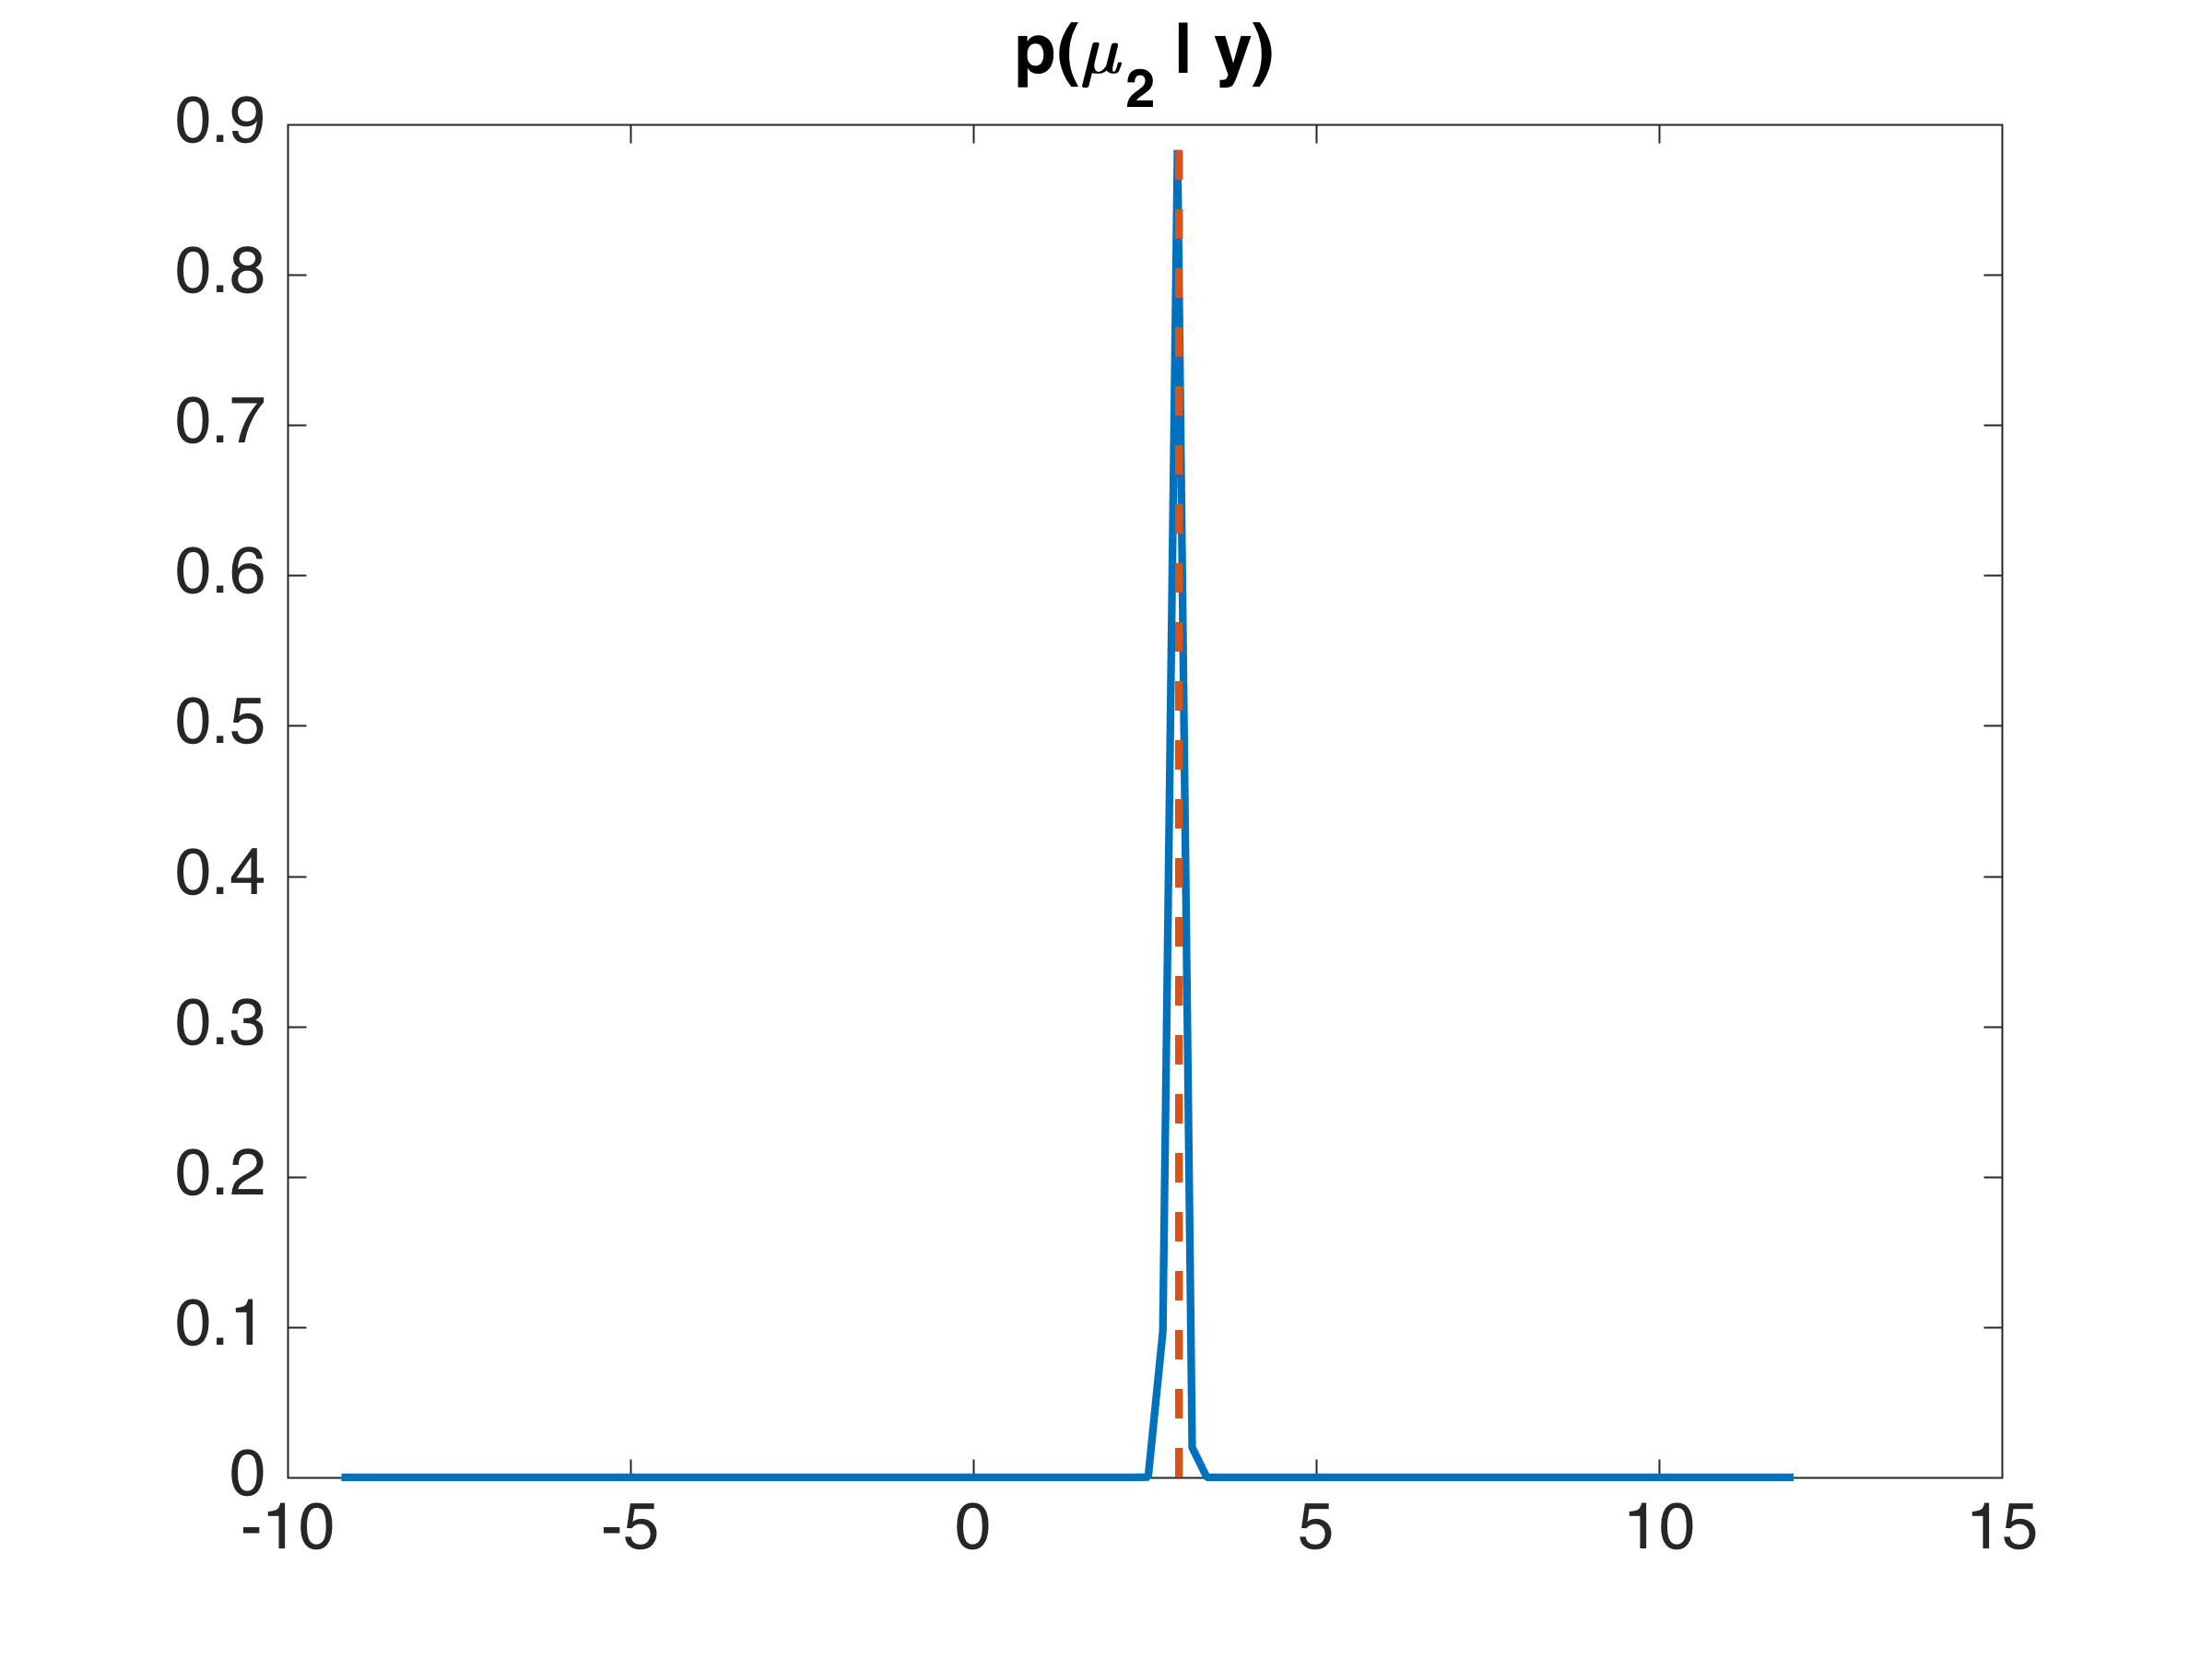
\includegraphics[width=0.9\textwidth]{posterior_mu2.png}
		\caption{}
		\label{posterior_mu2}
	\end{subfigure}
	\caption{Estimation (en bleu) par KDE des densités a posteriori marginales $p(\mu_1 | \Vecy)$ (\ref{posterior_mu1}) et $p(\mu_2 | \Vecy)$ (\ref{posterior_mu2}) après 5 itérations de l'AMIS, comparaison avec les valeurs attendues (en rouge).}
\end{figure}

Les figures \ref{posterior_mu1} et \ref{posterior_mu2} permettent de représenter explicitement les résultats de l'estimation de $\mu_1$ et $\mu_2$ grâce au procédé d'\textit{estimation par noyau} ou \textit{kernel density estimation} (KDE): si $\theta^{(1)}, \theta^{(2)}, \dots, \theta^{(n)}$ est un échantillon issu d'une variable aléatoire $\VecTheta$, alors l'estimateur de $\VecTheta$ par la méthode KDE est donné par :

 \begin{equation}
	\widehat{f}_h(\theta) = \dfrac{1}{nh}\sum\limits_{i=1}^n K\left(\dfrac{\theta - \theta^{(i)}}{h}\right)
	\label{eq_KDE} 
 \end{equation} 
 où $K$ est un noyau arbitrairement choisi et $h$ est la fenêtre du noyau, qui règle le degré de lissage de l'estimation. $K$ est ici choisi comme étant gaussien centré réduit, un choix fréquent dans ce genre de démarche. De plus, comme l'illustre la figure \ref{fig_boxplot_mu12}, les estimations fournies par l'AMIS sont relativement robustes.
 
\begin{figure}[h!]
	\centering
	\begin{subfigure}[t]{0.5\textwidth}
		\centering
		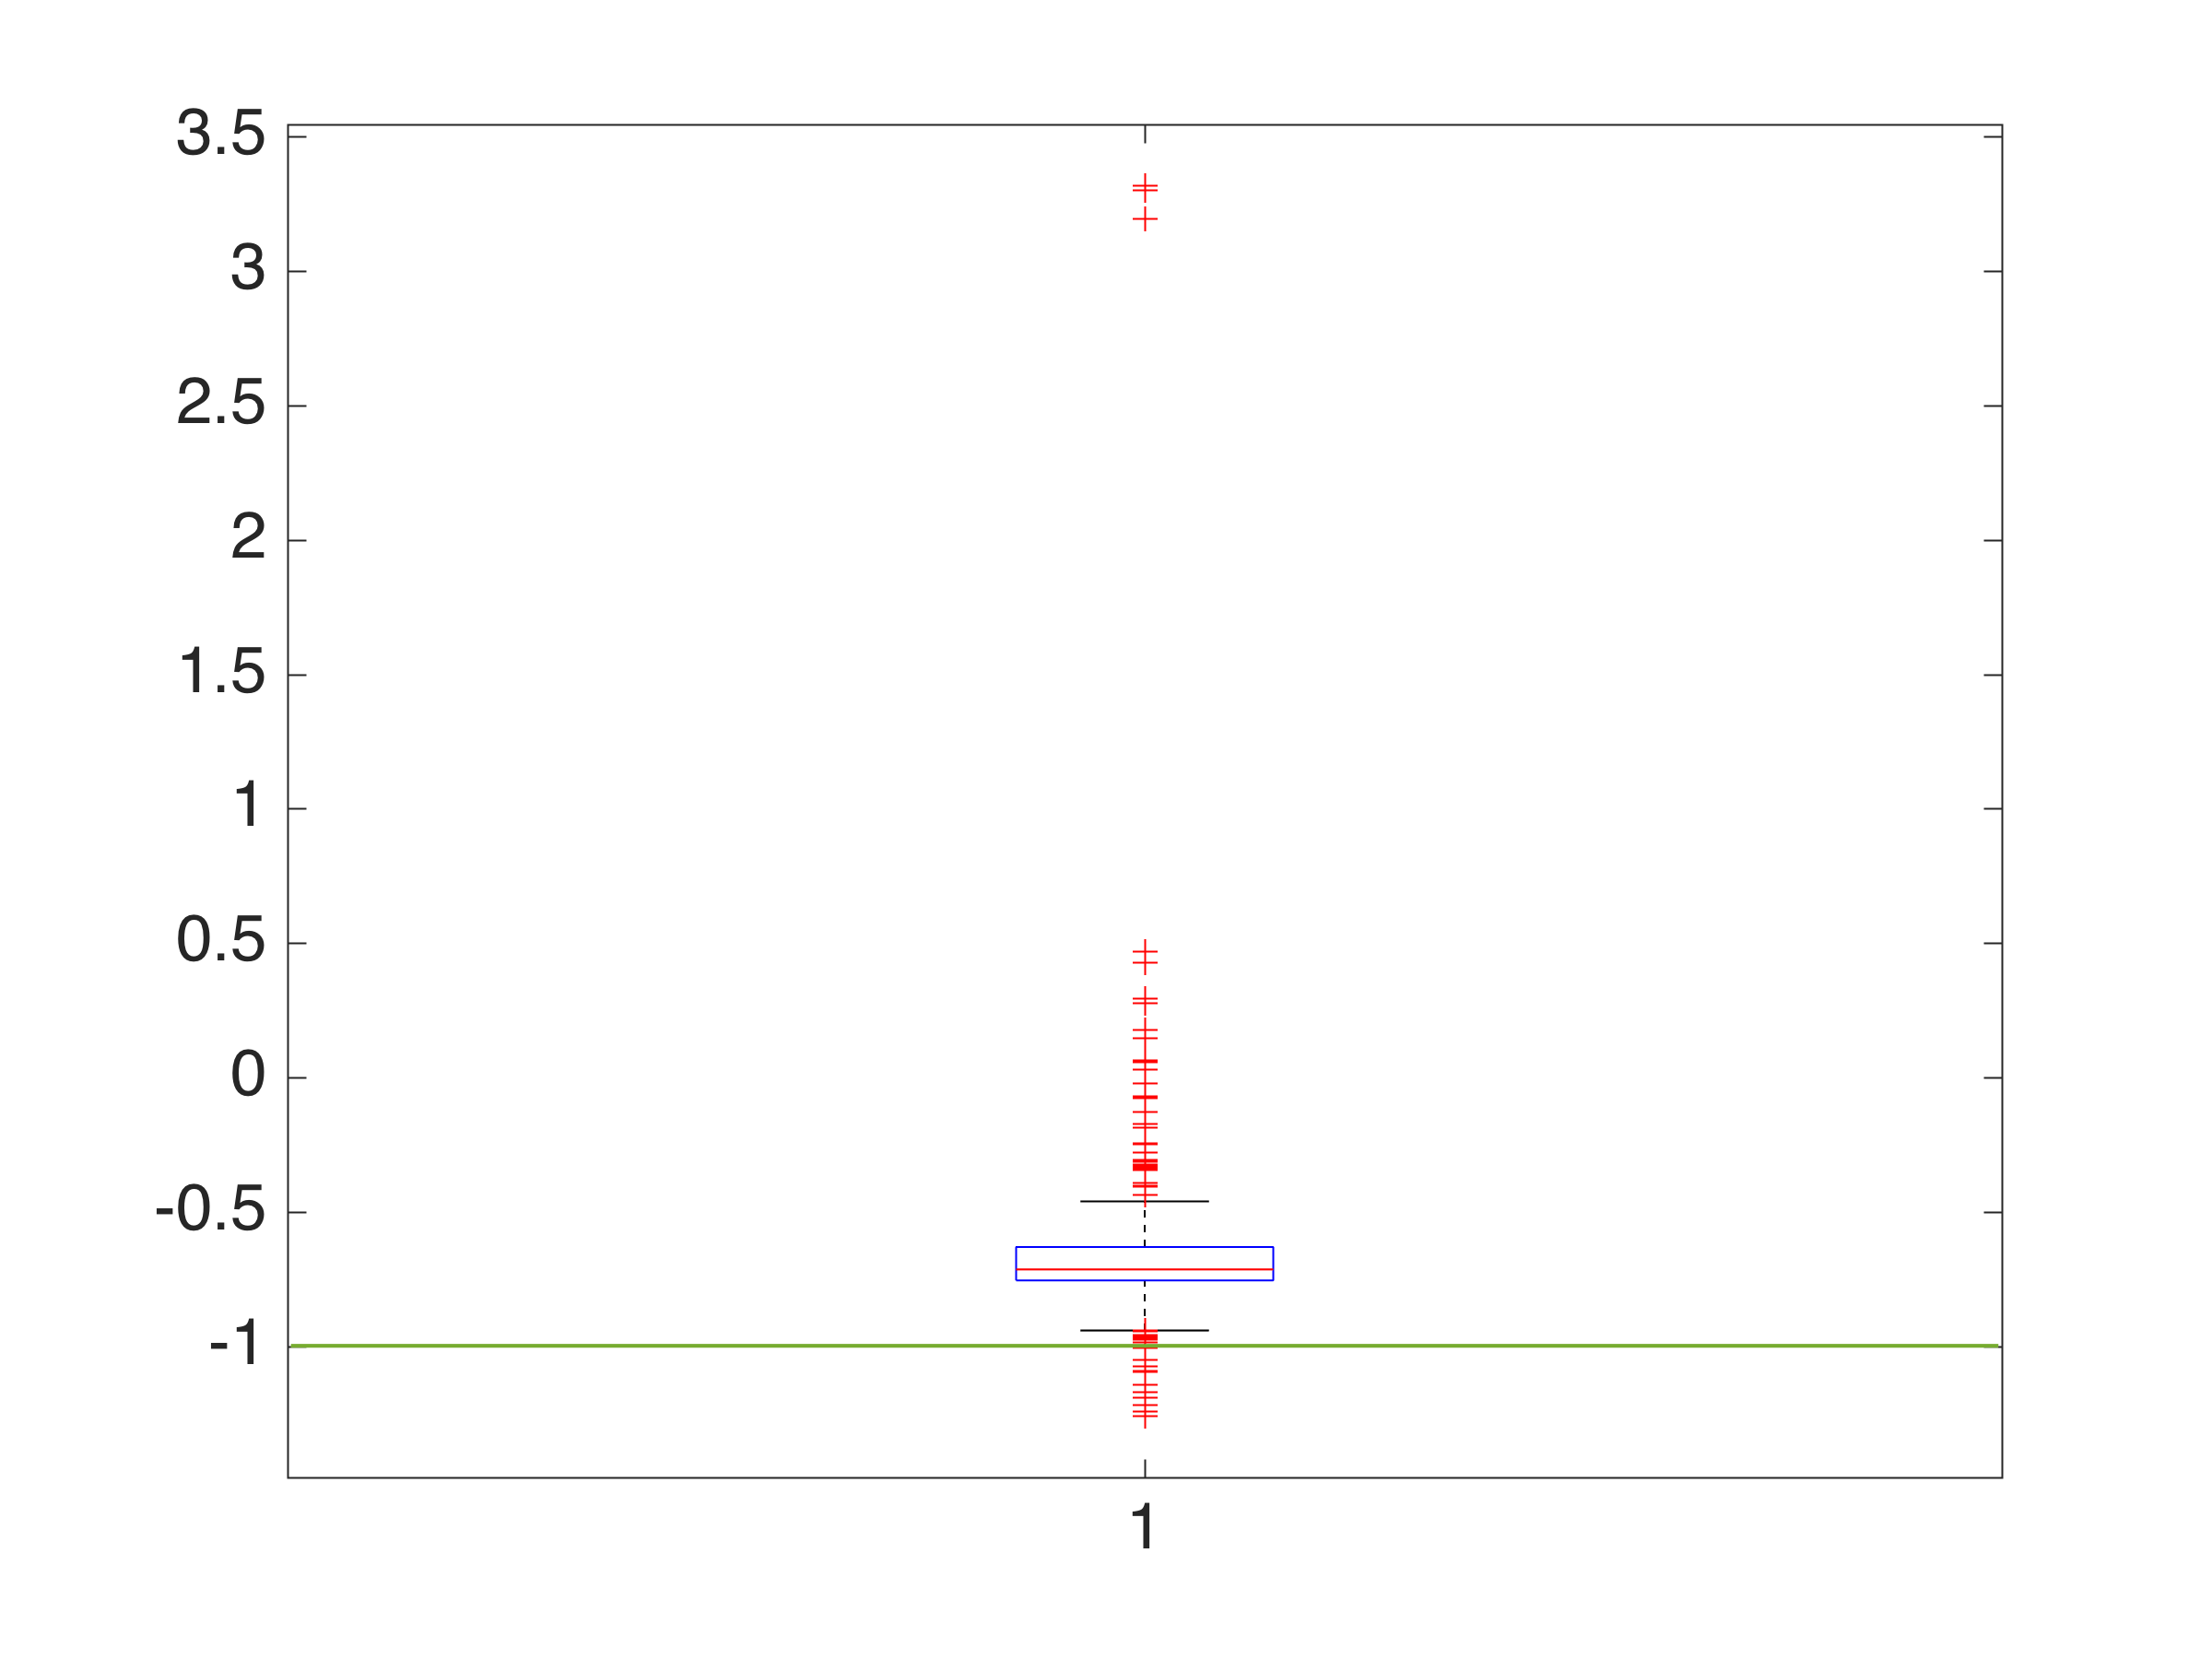
\includegraphics[width=0.9\textwidth]{boxplot_mmse_mu1}
		\caption{}
		\label{boxplot_mu1}
	\end{subfigure}%
	~ 
	\begin{subfigure}[t]{0.5\textwidth}
		\centering
		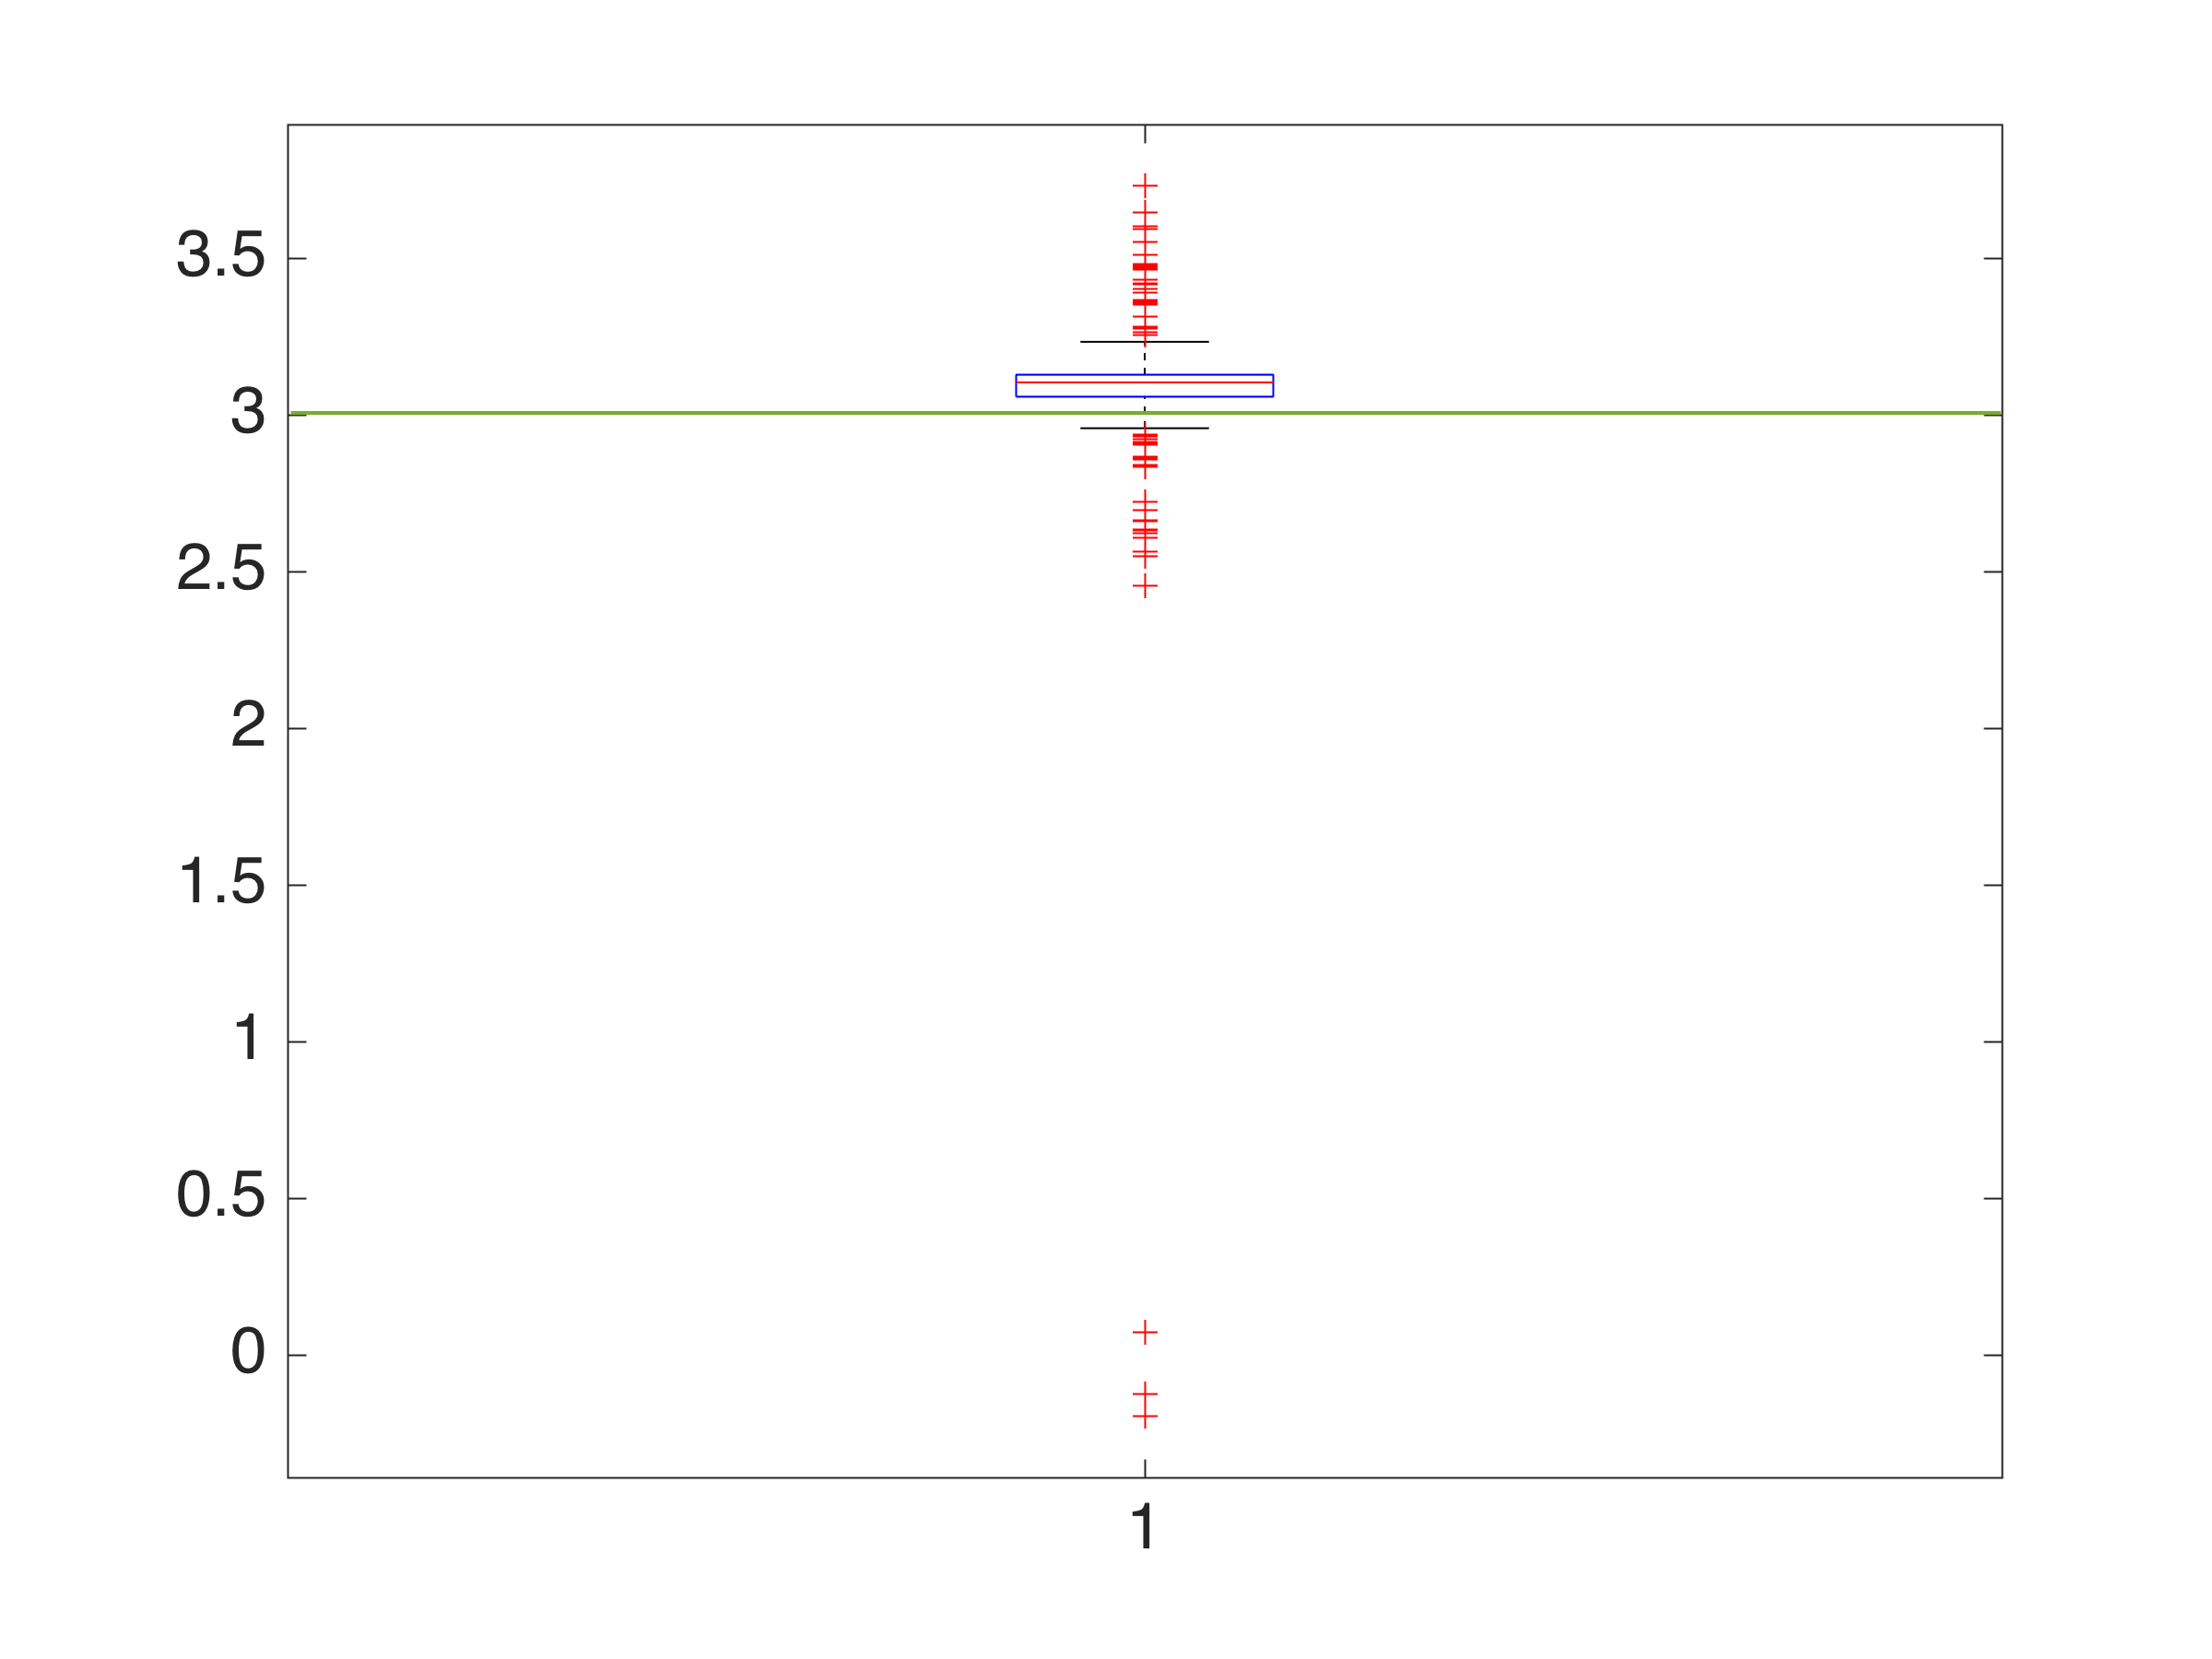
\includegraphics[width=0.9\textwidth]{boxplot_mmse_mu2}
		\caption{}
		\label{boxplot_mu2}
	\end{subfigure}
	\caption{Distribution statistique des estimateurs MMSE pour $p(\mu_1 | \Vecy)$ (\ref{boxplot_mu1}) et $p(\mu_2 |\Vecy)$ (\ref{boxplot_mu2}) pour 200 exécutions distinctes de l'algorithme, comparaison avec les valeurs attendues (en vert)}
	\label{fig_boxplot_mu12}
\end{figure}

Dans cet exemple, l'algorithme AMIS produit rapidement de bons résultats, l'incertitude étant légèrement plus élevée pour l'estimation de $\mu_1$ car de par la nature de la loi cible (modèle de mélange), comme $\rho=0.3$ seuls 30\% des observations sont représentatifs de la composante associée. \\

L'AMIS constitue ainsi une méthode aboutie pour l'échantillonnage d'importance adaptatif, c'est pourquoi son choix est privilégié pour l'application de l'inférence bayésienne à l'estimation du terme source dans la suite de ce manuscrit, plus particulièrement pour la localisation de la source. Les deux chapitres suivants présentent plus en détail sa mise en application sur différents types de cas pratiques. 



